%% Template para dissertação/tese na classe UFBAthesis
%% versão 1.0
%% (c) 2005 Paulo G. S. Fonseca
%% (c) 2012 Antonio Terceiro
%% (c) 2014 Christina von Flach
%% www.dcc.ufba.br/~flach/ufbathesis

%% Carrega a classe ufbathesis
%% Opções: * Idiomas
%%           pt   - português (padrão)
%%           en   - inglês
%%         * Tipo do Texto
%%           bsc  - para monografias de graduação
%%           msc  - para dissertações de mestrado (padrão)
%%           qual - exame de qualificação de mestrado
%%           prop - exame de qualificação de doutorado
%%           phd  - para teses de doutorado
%%         * Um­dia
%%           scr  - para verão eletrônica (PDF) / consulte o guia do usuário
%%         * Estilo
%%           classic - estilo original a la TAOCP (deprecated)
%%           std     - novo estilo a la CUP (padrão)
%%         * Paginação
%%           oneside - para impressão em face única
%%           twoside - para impressão em frente e verso (padrão)
\documentclass[bsc, classic, a4paper, oneside]{ufbathesis}
\DeclareMathAlphabet      {\mathbfit}{OML}{cmm}{b}{it}

%% Preambulo:
\usepackage{xcolor} 
%% This control colors of equations, tables, figures, links, references and etc.
\hypersetup{
  colorlinks,
  linkcolor={red!30!black},
  citecolor={blue!50!black},
  urlcolor={blue!80!black}
}
\usepackage[utf8]{inputenc}
\usepackage{graphicx,url}
\usepackage{caption}
\usepackage{lipsum}
\usepackage{amsmath}
\usepackage{mathtools}
\usepackage{enumitem}
\graphicspath{{assets/}}
\usepackage{algorithm2e}
\usepackage{qtree}
\usepackage{amstext} % Useful package to put accents in mathmode with \text
\usepackage{multirow}
\usepackage{array,booktabs}
%\everymath=\expandafter{\the\everymath\displaystyle}
\everymath{\displaystyle}
\SetKwRepeat{Do}{faça}{enquanto} % Macro to allow do while in algorithm2e
\SetKwBlock{Begin}{início}{fim}
\SetKwFor{For}{para}{faça}{fim} 
\SetKwFor{ForEach}{para cada}{faça}{fim} 
\SetAlgorithmName{Algoritmo}{Lista de Algoritmos}

% ---
% Citacao direta com mais de 3 linhas - ABNT NBR 10520/2002 - 5.3
\newlength{\ABNTEXcitacaorecuo}% recuo de 4 cm da margem esquerda
\setlength{\ABNTEXcitacaorecuo}{4cm}
\newcommand{\ABNTEXfontereduzida}{\footnotesize}
\newenvironment*{citacao}[1][default]
{
  \list{}%
  \ABNTEXfontereduzida%
  \addtolength{\leftskip}{\ABNTEXcitacaorecuo}%
  \item[]%
  %\begin{SingleSpace}%
  %\ifthenelse{\not\equal{#1}{default}}{\itshape\selectlanguage{#1}}{}%
}
{ 
  %\end{SingleSpace}%
  \endlist%
}


% Universidade
\university{UNIVERSIDADE FEDERAL DA BAHIA}

% Endereço (cidade)
\address{Salvador}

% Instituto ou Centro Acadêmico
\institute{INSTITUTO DE MATEMÁTICA}

% Nome da biblioteca - usado na ficha catalográfica
\library{BIBLIOTECA REITOR MAC\^{E}DO COSTA}

% Programa de pós-graduação
\program{Programa de Graduação em Ciência da Computação}

% Area de titulação
\majorfield{CI\^{E}NCIA DA COMPUTA\c{C}\~{A}O}

% Titulo da dissertação
\title{Uma abordagem híbrida para organização flexível de documentos}

% Data da defesa
% e.g. \date{19 de fevereiro de 2003}
\date{2 de junho de 2016}

% Autor
% e.g. \author{Jose da Silva}
\author{Nilton Vasques Carvalho Junior}

% Orientador(a)
% Opção: [f] - para orientador do sexo feminino
% e.g. \adviser[f]{Profa. Dra. Maria Santos}
\adviser[f]{Profa. Dra. Tatiane Nogueira Rios}

% Orientador(a)
% Opção: [f] - para orientador do sexo feminino
% e.g. \coadviser{Prof. Dr. Pedro Pedreira}
% Comente se não se aplicar
%\coadviser{NOME DO(DA) CO-ORIENTADOR(A)}

%% Inicio do documento
\begin{document}

\pgcompfrontpage{}

%% Parte pre-textual
\frontmatter

\pgcomppresentationpage

% Ficha catalográfica
\authorcitationname{Carvalho, Nilton Vasques Jr.} % e.g. Terceiro, Antonio Soares de Azevedo
\advisercitationname{Rios, Tatiane Nogueira} % e.g. Chavez, Christina von Flach Garcia
\catalogtype{Monografia (Graduação)} % e.g. ``Tese (Doutorado)''
\catalogtopics{``1. Fuzzy C Means. 2. Organização flexível de documents. 3. Lógica Fuzzy. 4. Mineração de dados.''} % e.g. ``1. Complexidade Estrutural. 2. Engenharia de Software''
\catalogcdd{NUMERO CDD} % e.g. ``CDD 20.ed. XXX.YY'' (esse número vai lhe ser dado pela biblioteca)
\catalogingsheet

% Termo de aprovação
\approvalsheet{Salvador, 02 de junho de 2016}{
   \comittemember{Profa. Dra. Tatiane Nogueira Rios}{Universidade Federal da Bahia}
   \comittemember{Prof. Dr. Maurício Pamplona Segundo}{Universidade Federal da Bahia}
   \comittemember{Prof. Dr. Ricardo Rios}{Universidade Federal da Bahia}
}

% Dedicatória
% Comente para ocultar
\begin{dedicatory}
Coloque sua DEDICATÓRIA AQUI.
\end{dedicatory}

% Agradecimentos
\acknowledgements
Coloque seus AGRADECIMENTOS AQUI.

% Epigrafe
%  \begin{epigraph}[Tarde, 1919]{Olavo Bilac}
%  Ultima flor do Lácio, inculta e bela,\\
%  Es, a um tempo, esplendor e sepultura;\\
%  Ouro nativo, que, na ganga impura,\\
%  A bruta mina entre os cascalhos vela.
%  \end{epigraph}
\begin{epigraph}[1687]{Isaac Newton}
  O que sabemos é uma gota, o que ignoramos é um oceano.
\end{epigraph}

% Resumo em Português
\resumo
O presente trabalho de conclusão de curso intenta realizar, à luz da literatura da área de mineração
de textos e campos do saber correlatos, uma investigação dos impactos dos algoritmos de agrupamento
na composição da organização flexível de documentos textuais. No seu princípio desta monografia,
discute-se a importância e as escolhas utilizadas na etapa pré-processamento, anterior à aplicação
do agrupamento, além dos critérios de validação do agrupamento que são utilizados no etapa do
pós-processamento, a saber, implementado pela medida da silheuta fuzzy. Para contextualizar a
prática da atividade de organização textual flexível proposta, destacam-se ao longo dos capítulos os
desafios inerentes à organização de textos, a exemplo o problema dos altos custos computacionais de
busca de graus de similaridade semântica em matrizes esparsas do tipo atributo valor, assim como os
possíveis mecanismos para mitigar ou reduzir os efeitos negativos dessas dificuldades no processo de
atribuição de significado aos grupos produzidos pelo agrupamento, através da extração de termos
descritores relevantes. A estratégia defendida aqui nesta monografia trata-se de uma abordagem
flexível e híbrida de organização de documentos, mesclando os benefícios concedidos pela adequada
interpretação de partições fuzzy e possibilísticas existentes no método de agrupamento Possibilistic
C-Means e Possibilistic Fuzzy C-Means (PFCM). Como fruto das análises experimentais aqui
desenvolvidas, foram propostos os métodos de extração de descritores Possibilistic Description Comes
Last (PDCL) e Mixed - Possibilistic Fuzzy Description Comes Last (PFDCL). Ambos mostraram-se
relevantes através de evidências experimentais e análises subjetivas à adequação dos métodos, para a
organização flexível de documentos, contribuindo com descobertas originais para o estado da arte da
área. Os resultados da pesquisa ainda estimulam novas implementações cuja execução pode se
transcorrer em trabalhos futuros.

% Palavras-chave do resumo em Português
\begin{keywords}
agrupamento fuzzy, agrupamento possibilístico, organização flexível de documentos, 
mineração de textos
\end{keywords}

% Resumo em Ingles
\abstract
The present coursework aims to conduct, under the knowledge of Text Mining and related areas, an
investigation about the impacts of clustering algorithms in the development of the flexible
organization of textual documents. In the beginning of this coursework, it is discussed the
relevance and the choices on  preprocessing stage, that is prior to clustering proper, besides, the
validation criteria of clustering during the post processing stage, namely, fuzzy silhouette. To
contextualize the piratical of the proposed flexible textual organization, it is remarked along
chapters the intrinsic challenges of text organization, for example, the  higher computational costs
problem in seeking semantic similarities degrees on sparse matrices value-attribute matrices, as
well as possible ways to mitigate or reduce the negative effects of these difficult on the process
meaning attribution groups that are outcome from clustering though relevant descriptors extraction
The strategy of the present course work consists in an approach of flexible and hybrid document
organization, mixing the benefits of the known fuzzy partition interpretation and possibilistic one
on clustering method of Possibilistic C-Means e Possibilistic Fuzzy C-Means (PFCM). As an output of
here developed experiments, it were proposed the Possibilistic Description Comes Last (PDCL) and
Mixed - Possibilistic Fuzzy Description Comes Last (PFDCL) descriptors' extraction methods.
Both were confirmed by experimental evidences and analysis that are subjective to methods adjusts
for the flexible organization of documents collaborating for original discoveries on the state of
arts. The results of the present research, after all, stimulate new implementations whose execution
may be executed on future works.

% Palavras-chave do resumo em Ingles
\begin{keywords}
fuzzy clustering, possibilistic clustering, flexible organization, documents, text mining
\end{keywords}

% Sumario / Índice
% Comente para ocultar
\tableofcontents

% Lista de figuras
% Comente para ocultar
\listoffigures

% Lista de tabelas
% Comente para ocultar
\listoftables

%% Parte textual
\mainmatter

% Eh aconselhável criar cada capitulo em um arquivo separado, digamos
% "capitulo1.tex", "capitulo2.tex", ... "capituloN.tex" e depois
% inclui-los com:
% \include{capitulo1}
% \include{capitulo2}
% ...
% \include{capituloN}
%
% Importante: Use \xchapter ao invés de \chapter, se quiser colocar texto antes do inicio do capitulo.

\xchapter{Introdução}{Uma breve introdução sobre do que se trata esta monografia e a maneira como o texto está organizado.}
\label{ch:intro}

%A new powerful and flexible organization of documents can be obtained by mixing fuzzy and
%possibilistic clustering, in which documents can belong to more than one cluster simultaneously
%with different compatibility degrees with a particular topic. The topics are represented by
%clusters and the clusters are identified by one or more descriptors extracted by a proposed method.
%We aim to investigate whether the descriptors extracted after fuzzy and possibilistic clustering
%improves the flexible organization of documents. Experiments were carried using a collection of
%documents and we evaluated the descriptors ability to capture the essential information of the used
%collection. The results prove that the fuzzy possibilistic clusters descriptors extraction is
%effective and can improve the flexible organization of documents.

O avanço da computação pessoal, em particular a computação móvel, tem proporcionado um gigantesco
aumento da quantidade de dados armazenados pela humanidade ao longo dos anos. A critério de exemplo,
a popular plataforma de rede social Facebook\footnotemark, produz diariamente mais de 25 $terabytes$
de informação \cite{Havens2012}. De acordo com \citeonline{Huang2015}, a tendência com o avanço das
tecnologias, é que tudo seja integrado a internet, de tal modo que os pesquisadores já chegam a
dizer que os dados são o novo recurso natural do planeta. Ainda segundo os autores,
entre as maiores fontes de geração de dados estão os sistemas governamentais, plataformas de mídias
sociais, assim como arquivos armazenados pelas corporações, como por exemplo, formulários médicos,
opiniões de consumidores, relatórios e etc.. Entretanto, \citeonline{Muggleton2006} ressalta que 
todos esses dados excedem os limites humanos para o uso e compreensão destes.
\footnotetext{\url{https://facebook.com/}}

Diante desse cenário, instituições públicas e privadas estão sobrecarregadas com a tarefa de
processar essa imensa quantidade de informação em bases de dados com documentos não estruturados e
em diversos formatos \cite{Kobayashi2008}. Estes documentos usualmente são de diversos tipos,
como por exemplo, textos, áudios, imagens, vídeos, documentos HTML, podendo estar, inclusive, em diferentes idiomas. 

Nesse contexto, diversas pesquisas tem objetivado a proposição ou refinamento de técnicas para
automatização do processo de análise e aquisição de conhecimento útil desse montante de informações
armazenadas. Porém, devido a multi disciplinaridade inerente desse campo de estudo, o mesmo tem
sido estudado pelas comunidades de mineração de dados, aprendizado de máquina e recuperação de
informação.

A Mineração de Dados (MD) é um campo de estudo que vem obtendo rápidos avanços nos últimos anos, e
segundo \citeonline{Aggarwal2012}, isto se deve aos avanços das tecnologias de $hardware$ e
$software$, o qual possibilitou o massivo armazenamento de diferentes tipos de dados, inclusive os
dados textuais. Portanto, como resultado desse aumento na quantidade de documentos disponíveis na
forma textual, existe uma demanda crescente no desenvolvimento e aprimoramento de métodos e
algoritmos que possam efetivamente processar e extrair padrões dos dados de maneira dinâmica e
escalável. 

Por outro lado, enquanto os dados estruturados já possuem mecanismos bem eficientes de armazenamento
e recuperação, os dados textuais são geralmente gerenciados através de mecanismos de buscas para
suprir essa falta de estruturação. Esses mecanismos de busca possibilitam aos usuários uma
conveniente maneira para recuperar informações em coleções textuais através de consultas com palavras
chaves. Desse modo, compete ao campo de estudo da Recuperação de Informação (RI) a tarefa de
explorar, investigar e propor métodos para otimização da eficiência e efetividade de
sistemas de buscas \cite{Baeza2011}. 

Mas segundo \citeonline{Baeza2011}, as pesquisas de recuperação de informação tem focado
tradicionalmente, em formas de facilitar o acesso à informação, do que realizar a descoberta de novos
padrões em documentos textuais, o qual se destaca como sendo o objetivo principal da mineração de
textos. A mineração de textos, por sua vez, é uma especialização da mineração de dados, que busca
incorporar atividades de estruturação dos documentos em formatos apropriados, facilitando a
aplicação dos tradicionais métodos de extração de padrões da MD, minimizando as perdas durante a
conversão do formato original não estruturado \cite{Nogueira2013}.

Contudo, uma série de características diferenciam os documentos textuais de outras formas de dados.
O que por sua vez, afeta o desempenho das clássicas técnicas da MD.  Dentre essas características
peculiares, destacam-se como mais importantes os fatos de que os dados são esparsos e possuem alta
dimensionalidade. Por exemplo, uma coleção de documentos (corpus) pode conter 100.000 palavras (termos), enquanto um único documento desse corpus pode conter somente algumas centenas de palavras \cite{Aggarwal2012}.  Essa discrepância,
tem implicações diretas em várias técnicas de identificação de padrões, e especialmente no
agrupamento textual, que deriva de clássicas técnicas de agrupamento da mineração de dados,
aplicados à conjuntos de baixa dimensionalidade. 
%estruturados. Com isso é notória a importância, de organizar de maneira automatizada, esses
%documentos pelos assuntos ao qual se tratam.

Para cumprir a tarefa de extrair informações relevantes de documentos textuais e identificar as
estruturas inerentes aos mesmos. A mineração de textos emprega uma variedade de técnicas, as quais se
destacam aquelas usualmente desenvolvidas para efetuar tarefas de coleta, pré-processamento, agrupamento textual e seleção de termos descritores para o agrupamento. 

O agrupamento pode, de maneira geral, ser definido como a tarefa de agrupar uma coleção de objetos,
de acordo algum critério de similaridade. É possível distinguir os tipos de agrupamento em
função da lógica empregada por eles. Com isso, tem-se os algoritmos que derivam da lógica clássica ou
da lógica fuzzy. Na lógica clássica, após a conclusão do agrupamento, cada elemento só pertence à
apenas um grupo, enquanto que na lógica fuzzy, a pertinência do elemento será distribuída entre os
grupos. 

Ao se analisar a diversidade de conteúdo em dados textuais, é trivial notar que frequentemente
um texto aborda um ou mais temas. O que implica que o agrupamento clássico, ao atribuir um objeto a
apenas um grupo, não irá representar bem a imprecisão e incerteza natural dos documentos. 

Deste modo, os métodos de agrupamento derivados da lógica fuzzy se mostram mais capacitados para
lidar com essa imprecisão e incerteza da realidade multi temática dos documentos textuais. Assim
sendo, uma organização flexível de documentos pode ser definida como o processo que compreende a
estruturação dos dados, a adição de flexibilidade proporcionada pelo agrupamento fuzzy, a extração
de descritores dos grupos de maneira flexível e a recuperação de informação através de um Sistema de Recuperação de Informação (SRI).

Ao se observar o processo de organização flexível de documentos, percebe-se que o mesmo abrange
várias etapas, cada uma delas com suas particularidades. No entanto, apesar da importância
desempenhada por cada etapa do processo, o agrupamento em si pode ser visto como uma das peças
chaves, pois ele é diretamente responsável por organizar os documentos de acordo com as suas
similaridades. Adicionalmente, é preciso desconsiderar ou reduzir a influência de
documentos ruidosos, que destoam do restante da coleção nos grupos finais.

Os algoritmos Fuzzy C-Means (FCM) \cite{Bezdek1984}, que deriva do clássico K-Means
\cite{Macqueen1967}, e o Possibilistic C-Means (PCM)
\cite{Krishnapuram1993}, são exemplos de métodos de agrupamento capazes de organizar de maneira
automatizada uma coleção de documentos em um conjunto de grupos
\cite{Mei2014,Tjhi2009,Prade2008,Saracoglu2008}. Ambos distribuem os documentos de uma coleção
textual em um conjunto de grupos, de modo que cada documento possa pertencer a diferentes grupos com
diferentes graus de pertinência, considerando assim a flexibilidade necessária para tratar a
imprecisão e incerteza do processo.

No entanto, o FCM apresenta alguns resultados indesejados, diante da presença de dados ruidosos na
coleção. Em se tratando de coleções textuais, um dado ruidoso pode ser considerado como um
documento que possua uma temática bastante diferente dos demais documentos da coleção. Com o
objetivo de atribuir valores de pertinências mais realísticos aos elementos a serem agrupados e
penalizar com baixas pertinências os elementos ruidosos, o algoritmo PCM foi proposto. Porém, o PCM
é muito sensível à inicialização, o que pode resultar em grupos coincidentes, onde não há uma
separação muito bem definida dos elementos.

Visando contemplar os benefícios de ambos os métodos, foi proposto o método de agrupamento Possibilistic Fuzzy C-Means
(PFCM) \cite{Pal2005}, como uma versão híbrida dos algoritmos FCM e o PCM,
objetivando adicionar robustez à tarefa de agrupamento.

Após o agrupamento dos documentos, é necessário realizar a extração dos termos que melhor descrevem
os grupos. Para realização dessa tarefa, tem-se alguns métodos na literatura do tipo DCF ({\it
Description Comes First}), que realizam a extração de maneira embutida no processo de agrupamento.
Porém, essa abordagem torna o processo de extração de descritores dependente do algoritmo de
agrupamento. Com o propósito de contornar esse cenário, foi proposto em \citeonline{Nogueira2013} o
método {\it Soft Organization - Fuzzy Description Comes Last} (SoftO-FDCL) \cite{Nogueira2013}, o qual extrai os termos descritores após a etapa de agrupamento de maneira independente do algoritmo de agrupamento utilizado. Permitindo avaliar diretamente os impactos dos métodos de agrupamento, na
extração de descritores e por consequência na qualidade da organização flexível de documentos.

Entretanto, o método SoftO-FDCL foi pensado inicialmente para interpretar as pertinências produzidas
na partição do FCM, que difere da partição resultante produzida pelo PCM. A principal contribuição
do PCM foi uma alteração no modo de atribuição da pertinência de uma elemento a um grupo, o que
impacta diretamente na partição dos grupos resultantes. 

Diante deste contexto, e tendo em vista o crescente aumento de informações produzidas além da capacidade humana de
analisar. Com a demanda crescente no desenvolvimento e aprimoramento das técnicas de extração e
identificação de conhecimento útil em dados textuais, bem como a necessidade de se organizar esses dados de
maneira flexível, tratando a imprecisão e incerteza natural desses dados e considerando as
particularidades existentes nos métodos de agrupamento, foi formulada a seguinte hipótese para o desenvolvimento desse trabalho:

\begin{quote}
\textit{A utilização de uma estratégia híbrida de agrupamento e extração de descritores, entre os 
  graus de pertinência e tipicidade providos pelo método de agrupamento PFCM, permitem o aumento da
    robustez e resiliência contra ruídos na organização flexível de documentos, aumentando assim a
    relevância dos grupos obtidos.}
\end{quote}

Para demonstrar a validade da hipótese formulada, com base na exploração de estratégias existentes
na literatura para o aprimoramento do processo de organização flexível de documentos, definiu-se o seguinte objetivo: 

\begin{quote}
\textit{Conduzir uma investigação em torno dos métodos de agrupamento FCM, PCM e PFCM, para
compreender e interpretar corretamente as peculiaridades de se extrair descritores a partir de um
agrupamento híbrido.}
\end{quote}

A fim de atender a esse objetivo, foram realizadas as seguinte tarefas ao longo do desenvolvimento desta monografia: estudo dos fundamentos teóricos necessários para a organização flexível de documentos, revisão das estratégias recentes
utilizadas por pesquisadores para aprimorar a organização flexível de documentos, condução de diversos experimentos para analisar os impactos da aplicação do algoritmo PFCM no processo de agrupamento e na extração de descritores.

Considerando-se os resultados dos experimentos realizados, foi descoberto que as alterações existentes no PCM, impactam diretamente na qualidade dos descritores extraídos pelo método SoftO-FDCL. Essa descoberta motivou a proposição de dois novos métodos de extração de descritores: {\it Possibilistic Descriptor Comes Last\/} (PDCL) e {\it Mixed - Possibilistic Fuzzy Descriptor Comes Last\/} (Mixed-PFDCL). Os quais apresentaram resultados que
contribuem de maneira significativa para o estado da arte da extração de descritores dos grupos
fuzzy e para o aprimoramento da organização flexível de documentos.

Detalhes de cada tarefa realizada, bem como a comprovação da hipótese levantada, são apresentados ao longo deste trabalho como segue:

{\bf Capítulo \ref{ch:theory}\/}: Neste capítulo, os fundamentos teóricos necessários para compreender o processo de organização flexível de documentos são apresentados, os quais contemplam a descrição da
etapa de pré-processamento e estruturação dos dados; a definição dos principais algoritmos de
agrupamento, capazes de proporcionar flexibilidade ao processo de organização de documentos; e a descrição da extração de
descritores.

{\bf Capítulo \ref{ch:related}\/}: Este capítulo aborda uma breve revisão do estado da arte encontrado
na literatura, referente às diversas estratégias propostas pelos pesquisadores. Com o objetivo de
aprimorar todas as etapas da organização flexível de documentos. 

{\bf Capítulo \ref{ch:proposed}\/}: Neste capítulo, um estudo dos impactos da
utilização do método de agrupamento híbrido na organização flexível de documentos é apresentado por meio da realização de análises experimentais. Neste capítulo, as influências das tipicidades presentes
na partição de pertinências do PCM também são apresentadas. Seguidas pela proposta dos métodos PDCL e Mixed-PFDCL. 

{\bf Capítulo \ref{ch:conclusion}\/}: Por fim, este capítulo contempla as conclusões obtidas de todo o estudo
realizado nesta monografia, assim como discussões a respeito dos resultados obtidos nos
experimentos. Aqui também está apontada uma série de possibilidades de extensões que derivam desta
pesquisa. 


\xchapter{Fundamentação Teórica}{Este capítulo tem como objetivo fundamentar as bases necessárias dos campos de estudos utilizados nesta monografia.}
\label{ch:theory}

\section{Considerações iniciais}
A lógica fuzzy foi introduzida por Lofti \citeauthoronline{Zadeh1965} em \citeyear{Zadeh1965}, onde
o autor inicia a discussão definindo os conjuntos fuzzy, as quais constituem classes de objetos com
valores contínuos de pertinência. Cada conjunto é caracterizado por uma função de pertinência, a
qual atribui a cada objeto do conjunto um grau de pertinência que varia entre zero e um. As
operações matemáticas da teoria dos conjuntos, como inclusão, união, intersecção, complemento,
relação, etc., também são estendidas aos conjuntos fuzzy, assim como várias propriedades dessas
notações são definidas.

Uma das motivações para o uso da lógica fuzzy, vem da maneira como nosso cérebro classifica e rotula
o mundo real. Por exemplo, ao rotularmos uma pessoa como alta, estamos atribuindo ela ao grupo de
pessoas altas. Assim como quando nos expressamos sobre o quanto um determinado dia está fazendo
calor ou frio. O conjunto de pessoas altas ou dias frios, não se enquadra na sua totalidade na
lógica clássica, pois essa forma imprecisa de descrever o mundo a nossa volta desempenha um papel
fundamental na forma de pensar humana, assim como também nas áreas de reconhecimento de padrões,
comunicação e abstração \cite{Zadeh1965}.  Neste sentido, esta seção tem como propósito
contextualizar os principais aspectos da lógica fuzzy que a torna tão importante no contexto da
organização flexível de documentos. Ressalta-se, portanto, que definições mais aprofundadas sobre a
lógica fuzzy fogem do escopo desse texto.  Adicionalmente, além dos principais fundamentos
necessários para compreensão da abordagem apresentada neste documento, estão a atividade de
pré-processamento dos dados, cuja finalidade é filtrar e estruturar os dados para serem processados
nas etapas seguintes; os principais algoritmos de agrupamento fuzzy, presentes na literatura, com as
suas definições matemáticas e pseudo códigos; e, por fim, a tarefa de rotular os grupos
encontrados na etapa de agrupamento com os termos que melhor os representem, permitindo assim a
realização de consultas em Sistemas de Recuperação da Informação
(SRI).

\section{Conjuntos e Lógica Fuzzy}

\subsection{Definição de conjuntos fuzzy}

Seja X um espaço de objetos, com um elemento genérico {\it x\/}.  Sendo $X= \big\{x\big\}$.
Um conjunto fuzzy $A$ em $X$ é caracterizado por uma função de pertinência $f_A(x)$, a qual associa
a cada elemento de $X$ um número real presente no intervalo de $[0,1]$, sendo o valor de $f_A(x)$ a
representação do grau de pertinência de $x$ em $A$.

\subsection{Lógica fuzzy}

A lógica fuzzy é uma lógica multi valorada, onde os valores das variáveis pertencem ao intervalo de
$[0,1]$, enquanto na lógica clássica os valores verdades só possuem os estados 0 ou 1 (também
conhecido como valores {\it crisp\/}). Uma da mais importantes aplicações está no tratamento de
precisão e incerteza. O que nos permite modelar soluções mais adequadas para ambientes imprecisos e
incertos.  Antes da lógica fuzzy ser introduzida por \citeonline{Zadeh1965}, em 1930 Lukasiewics
\cite{Chen2000} desenvolveu a lógica n-valorada para $3 < n < \infty$, utilizando apenas os
operadores lógicos de negação $-$ e implicação $\Rightarrow$. Dado então um inteiro positivo, $n >
3$, a lógica n-valorada assume valores verdade pertencente ao intervalo $[0,1]$, definidos pela
seguinte partição igualmente espaçada: $$0 =  \frac{0}{n-1},
\frac{1}{n-1},\frac{2}{n-1},...,\frac{n-2}{n-1},\frac{n-1}{n-1} = 1$$ Para estender a lógica
n-valorada para uma lógica com infinitos valores $2 \leq n \leq \infty$, \citeonline{Zadeh1965}
modificou a lógica de Lukasiewics definindo os seguintes operadores lógicos: 

$$\bar{a} = 1 -a$$ 
$$a \wedge b = min\{a,b\}$$ 
$$a \vee b = max\{a,b\}$$ 
$$a \Rightarrow b = min\{1, 1+b-a\}$$ 
$$a \Leftrightarrow  b = 1 - |a-b|$$

O objetivo da lógica fuzzy é prover mecanismos para tratar imprecisão e incerteza, se baseando na
teoria de conjuntos fuzzy e usando proposições imprecisas, de modo similar a lógica clássica usando
proposições precisas baseadas na teoria dos conjuntos.  Para entender essa noção, observe a seguir
um mesmo exemplo pela ótica do raciocínio clássico e pela ótica das ferramentas usadas para
descrever imprecisão da lógica fuzzy.  

\begin{enumerate}[label=\alph*)] 
\item Todo texto com 100 palavras ou mais da área jurídica, tem como assunto o direito. 
\item O texto A com título ``as manifestações de junho'', tem 100 palavras da área jurídica.  
\item O texto B com título ``política nas universidades'', tem 99 palavras da área jurídica.  
\item O texto A tem como assunto o direito e o texto B não tem como assunto o direito.  
\end{enumerate} 

Essa série de proposições ilustra o raciocínio empregado na lógica clássica e, seguindo as regras de
inferência, conseguimos verificar que as sentenças estão corretas. No entanto, é fácil notar que a
sentença d) não expressa muito bem o nosso entendimento sobre a temática dos textos.  Seria comum
alguém substituir a sentença d), por: O texto B fala um pouco sobre direito.  Sendo assim é possível
adicionar a imprecisão comum no mundo real às sentenças anteriores, conforme reescrito a seguir.

\begin{enumerate}[label=\alph*)] 
\item Todo texto que tem entre 50 e 100 palavras da área jurídica fala um pouco sobre direito.  Enquanto todo texto que contenha 100 ou mais palavras da área jurídica fala bastante sobre direito.  
\item O texto A com título ``as manifestações de junho'', tem 100 palavras da área jurídica.  
\item O texto B com título ``política nas universidades'', tem 99 palavras da área jurídica.  
\item O texto A fala bastante sobre direito, enquanto o texto B fala um pouco sobre direito. 
\end{enumerate} 

Esse tipo de dedução comumente utilizada no nosso dia a dia, não tem como ser tratada pela lógica
clássica. No entanto, podemos lidar com esse tipo de inferência imprecisa, empregando a
lógica fuzzy, a qual permite o uso de alguns termos linguísticos imprecisos como:
\begin{itemize} 
\item Predicados fuzzy: antigo, raro, caro, alto, rápido 
\item Quantificadores fuzzy: muito, pouco, quase, alguns 
\item Graus de verdade fuzzy: totalmente verdadeiro, verdadeiro, parcialmente falso, falso, definitivamente falso 
\end{itemize}

\section{Pré-Processamento} Pré-processamento dos dados é o processo de limpeza e preparação dos
dados para extração de padrões.  Para este trabalho, especificamente, considera-se dado como sendo
um documento textual e a tarefa de extração de padrões a ser considerada é o agrupamento.

Essa etapa é importante porque algumas palavras em um documento podem causar pouco ou nenhum impacto
no significado geral do documento \cite{Haddi2013}.  Soma-se a isso o enorme custo computacional do
processo de mineração de textos, devido à grande quantidade de atributos presente em dados
textuais, visto que quanto maior for a coleção de textos, maior será a quantidade de palavras
distintas. Tal dimensionalidade eleva bastante o custo computacional de qualquer tarefa de extração
de padrões.  Por isso, vários pesquisadores propuseram métodos para tentar simplificar, sintetizar e
eliminar redundâncias desnecessárias nas coleções de textos.  

A fase de pré-processamento voltada para a mineração de textos, as quais visam preparar dados
estruturados para as clássicas operações de mineração de dados, requer técnicas muito específicas
para o preparo dos dados não estruturados \cite{Feldman2007}.

Segundo \citeonline{Feldman2007}, é possível categorizar de maneira clara as técnicas de
pré-processamento de textos em duas categorias, de acordo com as tarefas realizadas pela técnica e
através dos algoritmos e frameworks que a mesma utiliza. Por sua vez, as técnicas categorizadas
pelas suas tarefas, geralmente visam realizar a estruturação do documento através de tarefas e sub
tarefas.  Como por exemplo, realizar a extração de título e sub título de documentos no formato PDF.
No entanto, as demais técnicas de pré-processamento são derivadas de métodos formais, e incluem
esquemas de classificação, modelos probabilísticos e sistemas baseado em regras.

O processo de pré-processamento de dados textuais, inicia com um documento parcialmente estruturado
e avança incrementando a estrutura através do refinamento das características do documento e
adicionando novas \cite{Feldman2007}.  No contexto da mineração de textos, as características dos
documentos são as suas palavras\cite{Haddi2013}. Ao final do processo, as palavras mais relevantes
são utilizadas, e as demais são descartadas.

O processo como um todo envolve várias etapas, as quais pode-se elencar a remoção de espaços,
expansão de abreviações, remoção de $stopwords$, que são palavras que não possuem relevância no
significado geral do texto e geralmente são compostas por proposições, pronomes, artigos,
interjeições dentre outras\cite{Nogueira2013}. Assim como também o processo de $stemming$ ou
lematização, onde se busca encontrar o radical da palavra, visando assim remover palavras que
possuam significados similares. Ainda é possível usar as técnicas de NLP ($Natural Language
Processing$) para eliminar sinônimos. Por fim, é realizada a seleção de termos mais característicos
para toda a coleção \cite{Haddi2013}. 

Diversos métodos foram propostos visando capturar a importância dos termos em coleções textuais.
Sendo o método { \it Term Frequency Inverse Document Frequency\/ }(TF-IDF) um dos mais importantes e
frequentemente utilizado na literatura \cite{Haddi2013}. A definição da TF-IDF está na Equação
(\ref{eq:tfidf}), onde $n$ é o número de documentos da coleção, $DF$ o total de documentos que
possuem este termo e $FF$ ({\it frequency feature}) a frequência do termo no documento.

\begin{equation} 
  \varphi(t,d) = FF * log(\frac{N}{DF}) \label{eq:tfidf} 
\end{equation}

Como resultado final de todo o processo de pré-processamento, obtém-se a matrix $D$. Onde $D$
representa os $n$ documentos da coleção, sendo cada documento $d_{i}$, com $1 \leq i \leq n$, uma
linha da matriz $D$, definido como sendo $ d_{i} =
[\varphi(t_{1},d_{i}),\varphi(t_{2},d_{i}),\varphi(t_{3},d_{i}),...,\varphi(t_{k},d_{i})] $, onde
$t_{j}$ é um termo presente na coleção, com $1 \leq j \leq k$.

\section{Agrupamento Fuzzy} 

O agrupamento é um processo não supervisionado cujo o objetivo é organizar os objetos similares no
mesmo grupo e os objetos com grau de dissimilaridade elevado em grupos distintos
\cite{Nogueira2013}. Este processo é de grande utilidade para diversos campos de estudo da
inteligência computacional, como a mineração de dados, recuperação de informação, segmentação de
imagens e classificação de padrões. Neste trabalho, os objetos a serem agrupados são os documentos
textuais.

O problema de organizar os documentos de maneira a maximizar a similaridade entre os membros de um
mesmo grupo, e minimizar a similaridade entre documentos de grupos distintos, é essencialmente um
problema de otimização.  Sendo assim, pretende-se otimizar a escolha dos grupos, entre
todas as possibilidades de agrupamento, dada uma função objetivo que captura a qualidade dos grupos.
Esta função é responsável por atribuir ao conjunto de possíveis grupos um número real, de maneira
que quanto melhor for os grupos, maior será o seu valor\cite{Feldman2007}.

A medida de similaridade desempenha um papel fundamental no agrupamento, uma vez que ela precisa
expressar o quão distante está um elemento do outro na coleção. Assim sendo, para obtermos bons
resultados durante o processo de agrupamento é de grande importância a escolha adequada da medida
de similaridade, e esta escolha precisa ser feita de acordo com o tipo dos dados.  Na literatura, a
medida de similaridade mais popular é a distância euclidiana (Equação
\ref{eq:euclidiana}), que tem se mostrado bastante adequada em dados com baixa dimensionalidade.

\begin{equation} 
  D(x_{i}, x_{j}) = \sqrt{\sum_k{(x_{ik}-x_{jk})^2}} 
  \label{eq:euclidiana}
\end{equation}

No entanto, em coleções textuais a matriz documentos x termos é naturalmente esparsa, devido a
grande variedade de termos em uma coleção, o que faz com que um determinado documento $d_{i}$ não
contenha diversos termos presentes em um outro documento $d_{j}$. Assim, o vetor de
características de cada documento acaba sendo preenchido com vários zeros, reduzindo a eficácia da
distância euclidiana (Equação \ref{eq:euclidiana}) \cite{Nogueira2013}. 

A medida de similaridade mais comum para coleções textuais é o coeficiente de similaridade de cosseno
\cite{Feldman2007}.  Por sua vez o coeficiente de similaridade de cosseno,
desconsidera os diversos zeros presentes nos vetores de termos dos documentos, levando em conta
apenas o ângulo formado entre eles\cite{Nogueira2013}.  Na Equação (\ref{eq:simcos}) temos a
definição do coeficiente de similaridade de cosseno, onde $d_1$ e $d_2$, são dois documentos
quaisquer da coleção de documentos, e $1 \leq t \leq k$, onde $k$ é a quantidade total de termos da
coleção, e $d_{ik}$ a frequência do termo $t$ no documento $d_i$.

\begin{equation} 
  scos(d_{1}, d_{2}) = cos\theta = \frac{d_{1} \cdot d_{2}}{|d_{1}||d_{2}|} =
  \sum_{t=1}^k{\varphi(d_{1t},d_1) \cdot \varphi(d_{2t},d_2)} \in [0,1] 
  \label{eq:simcos}
\end{equation}

Os grupos resultantes de um  processo de agrupamento, podem possuir algumas características que
estão diretamente relacionadas com o método de agrupamento empregado. Estes podem ser $hard$ ou
$crisp$, caso o método de agrupamento seja baseado na lógica clássica, assim como podem ser $soft$,
caso o método seja baseado na lógica fuzzy. No agrupamento $hard$, cada documento $d_{i}$ só poderá
pertencer a um único grupo $g_{j}$ \cite{Bezdek1984}. Enquanto em grupos $soft$, cada documento
$d_{i}$ pode pertencer a um ou mais grupos $g$, com grau de pertinência variados.  Além destes, os
grupos ainda podem ser $flat$ ou hierárquicos, onde no agrupamento $flat$ todos os grupos estão no
mesmo nível, enquanto no modelo hierárquico os grupos podem estar dispostos em uma hierarquia, de
modo que uma relação de parentesco é definida entre eles.

Para o agrupamento $hard$, considere $G = \{g_{1},g_{2},g_{3},...,g_{c}\}$ os grupos resultantes do
agrupamento, sendo $c$ o total de grupos, e a pertinência de cada documento $d_{i}$ à um grupo
$g_{l}$, $1 \leq l \leq c$, pode ser representada pela função característica $\kappa(d_{i}, g_{j})
\in \{0,1\}$.  Um dos mais populares algoritmos a implementar essa abordagem é o K-Means. Nos
trabalhos de \citeonline{Bezdek1984,Nogueira2013,Feldman2007}, é apontada uma falha inerente dessa
abordagem, pois quando um documento só pode pertencer a um único grupo, fica evidenciado que o mesmo
não compartilha nenhuma similaridade com os documentos dos demais grupos, o que não expressa a
imprecisão intrínseca da sobreposição dos assuntos em documentos de texto.

Com o objetivo de tratar essa falha da abordagem $hard$ e adicionar o tratamento de imprecisão e
incerteza no agrupamento, \citeonline{Bezdek1984} utilizou o modelo de partições fuzzy definido em
\citeonline{Zadeh1965}, para permitir pertinências parciais de um elemento a um grupo, propondo
assim o algoritmo Fuzzy C Means (FCM).  Sendo assim, a função característica passa a ser considerada
como uma função de pertinência de um documento $d_{i}$ em um grupo $g_{l}$, a qual é definida por
$\mu(d_{i}, g_{l}) \in [0,1]$, tal que $\sum_{l=1}^c \mu(d_{i}, g_{j}) = 1$.

Um desafio sempre presente em métodos de agrupamento é a descoberta do número ideal de grupos em uma
coleção. O método de organização flexível proposto em \citeonline{Nogueira2013}, utiliza a  $Fuzzy\
Silhouette$ (FS) para realizar a validação do agrupamento fuzzy, e por conseguinte encontrar o
número de grupos ideal. A função FS é uma adaptação do método de critério de largura média
($Average\ Silhuette\ Width\ Criterion$ - ASWC), desenvolvido para o agrupamento $crisp$. A
definição da silhueta fuzzy está nas Equações (\ref{eq:silhuette}) e (\ref{eq:fs}), onde
$\alpha(d_i, g_l)$ é a distância média entre o documento $d_i$ e todos os documentos presentes no
grupo $g_l$, enquanto $\beta(d_i,g_l) = min\{\alpha(d_i,g_h) | 1 \leq h \leq c; h \neq l\}$, é a
medida de dissimilaridade de $d_i$ ao grupo vizinho mais próximo de $g_l$, tal que $c$ é a
quantidade de grupos.  


\begin{equation} 
  S(d_i) = \frac{\beta(d_i, g_l) - \alpha(d_i,g_l)}{max\{\alpha(d_i,g_l), \beta(d_i,g_l)\}} 
  \label{eq:silhuette}
\end{equation}

\begin{equation} 
  FS = \frac{\sum_{i=1}^n{(\mu_1(d_i) - \mu_2(d_i))}S(d_i)}{\sum_{i=1}^n{(\mu_1(d_i) - \mu_2(d_i))}}
  \label{eq:fs}
\end{equation} 

Na Equação (\ref{eq:fs}), $\mu_1(d_i)$ é a maior pertinência do documento $d_i$ em um grupo,
enquanto $\mu_2(d_i)$ é a segunda maior. Quanto maior então for o valor da função FS, melhor será o
agrupamento. Deste modo, para encontrar o número de grupos ideal, basta executar a função FS
variando o número de grupos, e selecionar o agrupamento que tiver o valor máximo de FS.

Toda investigação realizada neste trabalho tomou como base os métodos de agrupamento que derivam do
algoritmo FCM\cite{Bezdek1984}, descrito a seguir, para se beneficiar da capacidade de tratar
imprecisão e incerteza da lógica fuzzy, e por conseguinte permitir que um mesmo documento seja
categorizado em mais de um tópico (grupo), refletindo a realidade dos documentos textuais. 

Em todos os experimentos a medida de similaridade de cosseno (Equação \ref{eq:simcos}) foi
utilizada, e a quantidade de grupos ideal foi escolhida utilizando o método da silhueta fuzzy (
Equação \ref{eq:fs}).

\subsection{Algoritmo Fuzzy C Means (FCM)} 

\citeonline{Bezdek1984} descreve um método de agrupamento fuzzy
que produz como saída partições fuzzy e protótipos dos grupos. Esse algoritmo desempenha um papel
importante no contexto do agrupamento fuzzy, devido ao seu pioneirismo no campo de estudo, possuindo
diversas extensões, sendo considerado um dos mais amplamente utilizados métodos de
agrupamento fuzzy da literatura\cite{Pal2005}. A maioria dos métodos de agrupamento fuzzy são
derivações do FCM\cite{Krishnapuram1993}.

Para compreensão do algoritmo, considere $V = \{v_1,v_2,v_3,...,v_c\}$ os protótipos dos grupos $G =
\{g_1,g_2,g_3,...g_c\}$ definidos por 

\begin{equation} 
  V = \left\{ v_j | v_j = \frac{\sum_{i=1}^n[\mu(d_i,g_j)]^m d_i}{\sum_{i=1}^n[\mu(d_i,g_j)]^m}, 
  1 < j \leq c \right\}, 
  \label{eq:prototipos} 
\end{equation}
tal que $v_j$ seja o protótipo de $g_j$, $c$ o número de grupos gerados no agrupamento e $n$ o
número de documentos presentes na coleção. 

Seja $U_{c \times n}$ uma partição fuzzy conforme a Equação:

\begin{equation} 
  U_{c \times n} = \{\mu(d_i, g_k) |\mu(d_i, g_k) \in [0,1], 1 < i \leq n, 1 < k \leq c\} 
  \label{eq:part_fuzzy} 
\end{equation} 

Esta partição apresenta todas as pertinências dos documentos aos grupos, cuja função de 
pertinência $\mu(d_i,g_k)$ de cada documento na coleção, é definida por 

\begin{equation} 
  \mu(d_i,g_k) = \frac{1}{\sum_{j=1}^n(\frac{dist(d_i,v_k)}{dist(d_i,v_j)})^{\frac{1}{m-1}}} 
  \label{eq:pertinencia}
\end{equation}
e está sujeita as restrições definidas nas equações (\ref{eq:fcmrestri1}) e (\ref{eq:fcmrestri2}).

Considera-se $m$ o fator de fuzificação, que regula o quão fuzzy será as partições finais. De modo
que para $m = 1$ a partição resultante é totalmente $crisp$ (Figura \ref{fig:cluster_crisp}) e para
$m \rightarrow \infty$ a interseção entre os grupos tende a aumentar (Figura
\ref{fig:cluster_fuzzy})\cite{Pal2005}. 

Segundo \citeonline{Bezdek1984} nenhuma teoria ou evidência computacional aponta para um valor ótimo
de $m$, contudo o autor aponta que a faixa de valores ideais aparenta ser $[1,30]$. Sendo assim, se
existir um conjunto de dados para teste, uma boa estratégia para a escolha de $m$ é a realização de
testes experimentais. Caso contrário, o intervalo de $[1.5, 3.0]$ aparenta trazer bons resultados
para a maior parte dos dados.

\begin{figure}[!htp] \centering 
   \begin{minipage}{0.45\textwidth} 
     \centering
    \includegraphics[width=0.6\columnwidth]{assets/clusters_crisp.pdf} 
    \caption{Ilustração denotando os
grupos $g_1,g_2,g_3$ organizados sem sobreposição, para $m = 1$.} 
  \label{fig:cluster_crisp}
  \end{minipage}\hfill 

  \begin{minipage}{0.45\textwidth} \centering
    \includegraphics[width=0.6\columnwidth]{assets/clusters_fuzzy.pdf} 
    \caption{Ilustração denotando os
     grupos $g_1,g_2,g_3$ organizados de maneira fuzzy, com sobreposição, quando 
     $m \rightarrow \infty$.}
     \label{fig:cluster_fuzzy} 
   \end{minipage} 
\end{figure}

Onde usualmente no contexto do agrupamento de coleções textuais $dist(d_i,g_k) = scos(d_i,g_k)$.
Adicionalmente, o algoritmo FCM estabelece algumas restrições: deve-se evitar que o FCM produza
grupos vazios (Equação (\ref{eq:fcmrestri1})) e deve-se impor que a soma das pertinências seja
sempre igual a um (Equação (\ref{eq:fcmrestri2})).

\leavevmode\\
\begin{equation} \sum_{k=1}^c
  \mu(d_i,g_k) = 1 \label{eq:fcmrestri1} 
\end{equation}

\begin{equation} 0 < \sum_{i=1}^n
  \mu(d_i,g_k) < n \label{eq:fcmrestri2} 
\end{equation}. 
\leavevmode\\

A restrição imposta pela Equação (\ref{eq:fcmrestri2}), no entanto, produz um problema em elementos
equidistantes aos grupos. Ou seja, quando temos o caso $\mu(d_i, g_1) = \mu(d_i, g_2) = ... =
\mu(d_i, g_c)$. Nessa situação, o grau de pertinência de um elemento a cada grupo será a pertinência
média, ou seja $\mu(d_i, g_1) = \mu(d_i, g_2) = ... = \mu(d_i, g_c) = \frac{1}{c}$. Supondo agora um
segundo documento $d_2$, que seja mais distante do que $d_1$, porém assim como $d_2$, também
equidistante aos grupos, temos que $\mu(d_2, g_j) = \mu(d_1, g_j) = \frac{1}{c}$, para $1 < j \leq
c$. Nesse contexto, a pertinência de $d_2$ e $d_1$, não expressa a distância relativa desses
documentos aos grupos. Esse problema está ilustrado na Figura \ref{fig:fcm_problem}.

\begin{figure}[!htp] \centering
  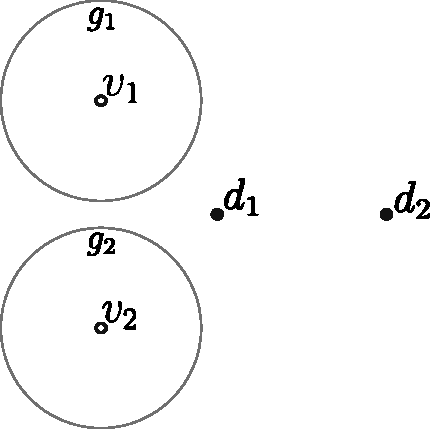
\includegraphics[width=0.4\columnwidth]{assets/fcm_problem.pdf} 
  \caption{Problema dos
    elementos equidistantes do algoritmo FCM. Na imagem $g_1$ e $g_2$ são grupos, com os seus
    respectivos protótipos $v_1$ e $v_2$. Enquanto $d_1$ e $d_2$ são documentos equidistantes aos
    protótipos $v_1$ e $v_2$. Portanto $\mu(d_1,g_1) = \mu(d_1,g_2) = \mu(d_2,g_1) = \mu(d_2,g_2) =
0.5$.} 
  \label{fig:fcm_problem} 
\end{figure}

Segundo \citeonline{Bezdek1984} várias funções de otimização da partição fuzzy produzida no
agrupamento foram propostas, sendo a minimização da função objetivo $J(U_{c \times n},G,V,D)$, 
definida na Equação (\ref{eq:fcm_obj}) a mais popular. Onde considere $U_{c \times n}$ como os graus
de pertinência fuzzy, $V$ os protótipos dos grupos $G$ e $D$ o conjunto de documentos.  

\leavevmode\\
\begin{equation} min\{(J(U_{c \times
n},G,V,D) = \sum_{i=1}^n \sum_{j=1}^c [\mu(d_i, g_j)]^m dist(d_i, v_j)\} 
\label{eq:fcm_obj}
\end{equation} 
\leavevmode\\

O algoritmo mais comumente utilizado para prover soluções aproximadas dessa minimização
(\ref{eq:fcm_obj}), é a através da iteração de Picard\footnotemark \cite{Pal2005} entre as equações
(\ref{eq:prototipos}) e (\ref{eq:part_fuzzy}). 
\footnotetext{Método iterativo para construção de soluções aproximadas, atribuído ao matemático
francês Charles Emile Picard (1856-1941).
\url{http://mathfaculty.fullerton.edu/mathews/n2003/PicardIterationMod.html}} 
O ciclo de aproximações se dá por $V_{t-1} \Rightarrow  U_t \Rightarrow  V_t$, onde, ao final de
cada iteração, é verificado se $\parallel V_{t-1} - V_t\parallel < \varepsilon$.  A literatura
também expressa que os ciclos podem começar pela partição fuzzy, fazendo então $U_{t-1} \Rightarrow
V_t \Rightarrow U_t$, e, ao final do ciclo, checando o erro mínimo com $\parallel U_{t-1} -
U_t\parallel < \varepsilon$, sendo $t$ o contador de iterações.  Contudo, existem benefícios em
termos de processamento e memória ao utilizar a iteração iniciando e finalizando com
$V$\cite{Pal2005}. Por outro lado, \citeonline{Bezdek1984} e \citeonline{Pal2005} afirmam que a
convergência desse modelo iterativo ocorre em ambos os tipos de ciclo. Geralmente, a partição fuzzy
inicial $U_0$ é comumente inicializada com valores aleatórios ou com o resultado de um agrupamento
previamente executado \cite{Pal2005,Krishnapuram1993}. Nas demais iterações a atualização dos
protótipos é realizada a partir da Equação (\ref{eq:prototipos}).  

O pseudo código utilizando a abordagem iterativa descrita a cima, está listado no Algoritmo
\ref{alg:fcm}, no qual a função $\textbf{{\color{blue}inicializa-particao-fuzzy}(D,G)}$, pode ser
uma das duas formas de inicialização descritas anteriormente.

\leavevmode\\
\begin{algorithm}[H] 
  \SetAlgoLined 
  \textbf{{\color{blue}fcm}(D, c, m, $\varepsilon$)}\\
  \Begin{
    G $\gets$ $[g_1,g_2,...,g_c]$\; 
    $U_0$ $\gets$ \textbf{{\color{blue}inicializa-particao-fuzzy}(D,G)}\; 
    $t \gets 0$\; 
    \Do{ $\parallel U_{t-1} - U_t\parallel > \varepsilon$ }{ 
      $V_t$ $\gets$ calcula usando (\ref{eq:prototipos})\; 
      $t \gets t + 1$\; 
      $U_t$ $\gets$ calcula usando (\ref{eq:part_fuzzy})\; 
    }
    $\textbf{retorne} (U_t, V_t)$\; 
  }
  \caption{Pseudo código da implementação iterativa do método FCM}
\label{alg:fcm} 
\end{algorithm} 
\leavevmode\\

Por fim, está ilustrado na Figura \ref{fig:samples_fcm}, os resultados produzidos pelo algoritmo
FCM, em dois conjuntos de coordenadas no $R^2$. Na figura, os pontos foram pintados com a cor
correspondente ao grupo em que o mesmo obteve o maior valor de pertinência.

\leavevmode\\
\begin{figure}[!htp] 
  \centering 
  \includegraphics[width=0.8\columnwidth]{assets/samples_fcm.png}
  \caption{Resultado do agrupamento de dois conjuntos de coordenadas no $R^2$ usando o algoritmo
  FCM\protect\footnotemark.} 
  \label{fig:samples_fcm} 
\end{figure}
\leavevmode\\

\subsection{Algoritmo Possibilistic C Means (PCM)}

A restrição probabilística do FCM, apresentada na Equação (\ref{eq:fcmrestri2}), que obriga a soma
das pertinências de um elemento ser igual a um, nem sempre resulta em pertinências que representam
bem a realidade dos dados, conforme exemplificado na Figura \ref{fig:fcm_problem}.  Esse problema se
agrava ainda mais, em bases com muitos dados ruidosos ($outliers$). Portanto, com o objetivo de
contornar esses problemas do FCM, foi proposto em \citeonline{Krishnapuram1993} o algoritmo
$Possiblistic\ C\ Means$ (PCM). 

Ao contrário do FCM, o PCM não atribui pertinências dos documentos aos grupos, mas sim tipicidades,
as quais podem ser interpretadas como graus de possibilidade de um elemento pertencer a um
determinado grupo. Como consequência, a partição resultante é possibilística. Para se adequar a essa
abordagem possibilística, a função objetivo do PCM deriva da Equação (\ref{eq:fcm_obj}) do FCM.
Tendo também as funções de atualização de protótipos e atribuição de pertinências modificadas.

Na teoria de conjuntos fuzzy, a pertinência de um elemento a um grupo fuzzy não depende da
pertinência desse mesmo elemento em outro grupo. No entanto, no modelo FCM, a restrição apresentada
pela Equação (\ref{eq:fcmrestri2}) torna dependente a pertinência dos elementos aos grupos. De
maneira que se um elemento obtiver um grau elevado de pertinência em um dado grupo, ele não poderá
ter uma pertinência também elevada em outro grupo. Ou seja $\mu(d_1, g_1) = 1-\mu(d_1,g_2)$, supondo
um agrupamento com dois grupos. Nesse contexto \citeonline{Krishnapuram1993} sugere relaxamento da
restrição, permitindo assim, que a pertinência dependa unicamente da distância do elemento ao grupo.
Logo, as restrições apresentadas nas Equações (\ref{eq:fcmrestri1}) e (\ref{eq:fcmrestri2}), são
redefinidas nas Equações (\ref{eq:pcmrestri1}) e (\ref{eq:pcmrestri2}), nas quais $\lambda(d_i,g_j)$
representa a tipicidade do documento $d_i$ em relação ao grupo $g_j$.

\leavevmode\\
\begin{equation}
  \lambda(d_i, g_j) \in [0,1], \forall i,j
  \label{eq:pcmrestri1}
\end{equation}

\begin{equation}
  0 < \sum_{j=1}^n \lambda(d_i, g_j) \leq n, \forall j
  \label{eq:pcmrestri2}
\end{equation}
\leavevmode\\

Com isso, se mantiver-se a função objetivo do FCM (Equação \ref{eq:fcm_obj}), seria possível obter
uma solução trivial, bastando atribuir $0$ à todas as pertinências para minimizar se a função
objetivo $J(U_{c \times n},G,V,D)$ \cite{Krishnapuram1993}.  Portanto, para evitar essa solução, e
manter a característica de se atribuir pertinências elevadas aos elementos representativos e
penalizar os elementos não representativos, os autores reformularam a função objetivo do FCM
conforme está apresentado na Equação \ref{eq:pcmobj}. No qual o parâmetro $\gamma_j$ regula o limiar
da distância dos documentos ao grupo $g_j$, de modo que se um documento tiver distância maior do que
$\gamma_j$ a sua tipicidade em relação ao $grupo_j$ será menor do que 0,5, e se a distância for
menor do que $\gamma_j$, o seu grau de compatibilidade no $grupo_j$ será maior do que 0,5.

\leavevmode\\
\begin{equation}
  K_m(P_{c \times n},G,V,D) = \sum_{j=1}^c \sum_{i=1}^n [\lambda(d_i, g_j)]^m dist(d_i, v_j) +
  \sum_{j=1}^c \gamma_j \sum_{i=1}^n [1 - \lambda(d_i, g_j)]^m
  \label{eq:pcmobj}
\end{equation}
\leavevmode\\

De acordo com \citeonline{Krishnapuram1993}, o valor de $\gamma_j$ deve ser escolhido a depender da
faixa de possibilidades (tipicidades) desejada para um grupo. Por exemplo, $\gamma_j$ pode ser igual
para todos os grupos, quando se deseja que o formato dos grupos seja similar.  Contudo, na maioria
dos casos, se espera que $\gamma_j$ reflita o formato e tamanho particular de cada grupo. Assim
sendo, os autores indicam que a definição apresentada na Equação (\ref{eq:pcmgamma}) tem se mostrado
adequada para maior parte dos dados, onde $L$ é usualmente 1. 

\leavevmode\\
\begin{equation}
  \gamma_j = L \frac{\sum_{i=1}^n \lambda(d_i,g_j)^m dist(d_i,v_j)}{\sum_{i=1}^n \lambda(d_i,g_j)^m}
  \label{eq:pcmgamma}
\end{equation}
\leavevmode\\

A partição de graus de compatibilidade possibilísticos do PCM está definida na Equação
(\ref{eq:pcmpart}), a qual $\lambda(d_i, g_k)$ é sujeita as restrições apresentadas nas Equações
(\ref{eq:pcmrestri1}) e (\ref{eq:pcmrestri2}). 

\leavevmode\\
\begin{equation} 
  P_{c \times n} = \{\lambda(d_i, g_k) |\lambda(d_i, g_k) \in [0,1], 1 < i \leq n, 1 < k \leq c\}
  \label{eq:pcmpart} 
\end{equation} 

\begin{equation}
  \lambda(d_i,g_j) = \frac{1}{1+\left(\frac{dist(d_i,g_j)}{\gamma_j}\right)^{\frac{1}{m-1}}}
  \label{eq:lambda}
\end{equation}
\leavevmode\\

Por sua vez, a atualização de protótipos do PCM, ocorre de maneira similar a Equação
(\ref{eq:prototipos}) do FCM, apenas alterando a pertinência $\mu(d_i,g_j)$ por $\lambda(d_i,g_j)$.

A síntese do algoritmo PCM está apresentada em forma de pseudo código no Algoritmo \ref{alg:pcm}. \\

\leavevmode\\
\begin{algorithm}[H] 
  \SetAlgoLined 
  \textbf{{\color{blue}pcm}(D,c,m,$\varepsilon$)}\\
  \Begin{
    G $\gets$ $[g_1,g_2,...,g_c]$\; 
    $P_0$ $\gets$ \textbf{{\color{blue}inicializa-particao-fuzzy}(D,G)}\; 
    $\gamma_j \gets$ calcula utilizando (\ref{eq:pcmgamma})\;
    $t \gets 0$\; 
    \Do{ $\parallel P_{t-1} - P_t\parallel > \varepsilon$ }{ 
      $V_t$ $\gets$ calcula usando (\ref{eq:prototipos})\; 
      $t \gets t + 1$\; 
      $P_t$ $\gets$ calcula usando (\ref{eq:pcmpart})\; 
    }
    $\textbf{retorne} (P_t, V_t)$\; 
  }
  \caption{Pseudo código da implementação iterativa do método PCM}
  \label{alg:pcm} 
\end{algorithm}
\leavevmode\\

Por fim, está ilustrado na Figura \ref{fig:samples_pcm_fcm} (a), o resultado do agrupamento
obtido pelo método FCM; e, em (b), o agrupamento gerado pelo algoritmo PCM em um conjunto de 
coordenadas no $R^2$. Na figura, os pontos foram pintados com a cor correspondente ao grupo em que o 
mesmo obteve o maior valor de pertinência. Observa-se nessa comparação simplificada que o algoritmo 
PCM tentou maximizar a pertinência dos pontos aos grupos maiores, ocasionando uma maior quantidade
de pontos com pertinência elevada em dois grupos, ao contrário do FCM que distribuiu de maneira
uniforme os pontos em 4 grupos.

\begin{figure}[!htp] 
  \centering 
  \includegraphics[width=0.8\columnwidth]{assets/samples_pcm_fcm.png}
  \caption{Demonstração de agrupamentos obtidos com os algoritmos 
    FCM\protect\footnotemark (a) e PCM\protect\footnotemark[\value{footnote}](b)
  .} 
  \label{fig:samples_pcm_fcm} 
\end{figure}
\footnotetext{Resultados obtidos baseados na implementação dos algoritmo FCM e PCM, produzida como
parte deste trabalho disponível em: \url{https://github.com/niltonvasques/fcm}}

\subsection{Algoritmo Possibilistic Fuzzy C Means (PFCM)} 

De acordo com \citeonline{Pal2005} o algoritmo PCM pode levar os resultados do agrupamento 
a conter grupos coincidentes. Ou seja, quando o protótipo $v_i$ está muito próximo de outro protótipo
$v_j$. Segundo os autores, isto ocorre quando a inicialização da partição inicial não possui 
protótipos
suficientemente separados. Esse problema não é causado por uma escolha ruim da penalidade presente
na função objetivo do PCM, o que ocorre é uma falta de restrições para evitar que isso aconteça.

\citeonline{Carvalho2016} cita que as pertinências do FCM e as tipicidades do PCM são ambas
importantes para a correta interpretação das sub estruturas dos dados. Quando se tem dados que
precisam ser agrupados de maneira $hard$, as pertinências se mostram como uma escolha adequada, de
modo que é intuitivo atribuir o elemento ao grupo em que o mesmo possua a maior pertinência. Por
outro lado, durante a atualização dos protótipos, as tipicidades desempenham um papel fundamental
para aliviar os efeitos indesejados dos dados ruidosos.

Com o propósito de aproveitar os benefícios de ambas as abordagens, \citeonline{Pal2005} propôs o
algoritmo PFCM, que utiliza as pertinências $\mu(d_i,g_j)$ do FCM e as tipicidades
$\lambda(d_i,g_j)$ do PCM. Cabe ao usuário definir a proporção de cada uma das contribuições com
parâmetros que ponderam o peso de ambos. Para tanto, é realizada uma mistura entre as funções
objetivo apresentadas nas Equações (\ref{eq:fcm_obj}) e (\ref{eq:pcmobj}) resultando na minimização
da função objetivo apresentada na Equação (\ref{eq:pfcmobj}), a qual está sujeita as condições
impostas pela Equação (\ref{eq:pfcmrestri}), onde $a,b > 0$ e $m,n > 1$. Por sua vez, os parâmetros
$a$ e $b$, representam a importância relativa dos valores de pertinência e tipicidades, os quais
ficam a critério do usuário a sua definição de acordo com o contexto dos dados. De maneira geral, os
autores sugerem que $b$ seja maior que $a$, porém não muito maior, para não eliminar completamente
os benefícios do FCM. 

\leavevmode\\
\begin{equation}
  L_m(U_{c \times n},P_{c \times n},G,V,D) = \sum_{j=1}^c 
  \sum_{i=1}^n [a\mu(d_i,g_j)^n + b\lambda(d_i, g_j)^m] dist(d_i, v_j) +
  \sum_{j=1}^c \gamma_j \sum_{i=1}^n [1 - \lambda(d_i, g_j)]^m
  \label{eq:pfcmobj}
\end{equation}
\begin{equation}
  \sum_{j=i}^c \mu(d_i,g_j) = 1, \forall i, 0 < \mu(d_i,g_j),\lambda(d_i,g_j) \leq 1
  \label{eq:pfcmrestri}
\end{equation}
\leavevmode\\

A mistura e as ponderações adicionados no algoritmo PFCM também são agregadas a função de
atualização dos protótipos apresentada na Equação (\ref{eq:pfcmproto}), a qual passa a se beneficiar
das características de ambos os algoritmos.  

\leavevmode\\
\begin{equation}
  V = \left\{ v_j | v_j = \frac{\sum_{i=1}^n[a\mu(d_i,g_j)^n + b\lambda(d_i, g_j)^m] d_i}
    {\sum_{i=1}^n[a\mu(d_i,g_j)^n + b\lambda(d_i, g_j)^m]}, 
  1 < j \leq c \right\} 
  \label{eq:pfcmproto}
\end{equation}
\leavevmode\\

Desta maneira, é minimizado os efeitos dos dados ruidosos do FCM, assim como também o problema
dos protótipos coincidentes do PCM e a singularidade do FCM é evitada. 

\begin{figure}[!htp] 
  \centering 
  \includegraphics[width=0.6\columnwidth]{assets/samples_pfcm.png}
  \caption{Demonstração do agrupamento obtido com os algoritmo 
    PFCM\protect\footnotemark em um conjunto de coordenadas de pontos no $R^2$.} 
  \label{fig:samples_pfcm} 
\end{figure}
\footnotetext{Resultados obtidos baseados na implementação
  dos algoritmo FCM e PCM, produzida como parte este trabalho disponível em: 
\url{https://github.com/niltonvasques/fcm}}

O pseudo código do PFCM é apresentado no Algoritmo \ref{alg:pfcm}, onde a função \\
$\textbf{\color{blue}inicializa-prototipos}(D,G)$ é responsável por gerar os protótipos iniciais
da partição $V_0$.

Como resultado demonstrativo desse algoritmo, é possível observar na Figura \ref{fig:samples_pfcm},
que os grupos produzidos são em certa perspectiva um intermédio entre o agrupamento produzido pelo
FCM e PCM no mesmo conjunto de dados, apresentados na Figura \ref{fig:samples_pcm_fcm}.

\leavevmode\\
\begin{algorithm}[H] 
  \SetAlgoLined
  \textbf{{\color{blue}pfcm}(D, c, m, $\varepsilon$)}\\
  \Begin{
    G $\gets$ $[g_1,g_2,...,g_c]$\; 
    $V_0$ $\gets$ \textbf{{\color{blue}inicializa-prototipos}(D,G)}\; 
    $\gamma_j \gets$ calcula utilizando a Equação (\ref{eq:pcmgamma})\;
    $t \gets 0$\; 
    \Do{ $\parallel V_{t-1} - V_t\parallel > \varepsilon$ }{ 
      $U_t$ $\gets$ calcula com Equação (\ref{eq:part_fuzzy}) usando $V_{t-1}$\; 
      $P_t$ $\gets$ calcula com Equação (\ref{eq:pcmpart}) usando $V_{t-1}$\; 
      $V_t$ $\gets$ calcula com Equação (\ref{eq:pfcmproto})\; 
      $t \gets t + 1$\; 
    }
    $\textbf{retorne} (U_t,P_t,V_t)$\; 
  }
  \caption{Pseudo código da implementação iterativa do método PFCM}
  \label{alg:pfcm} 
\end{algorithm}
\leavevmode\\

\subsection{Algoritmo Hierarchic Fuzzy C Means (HFCM)}

Documentos de texto tratam de vários temas, como política, esporte, tecnologia e etc.
E os métodos de agrupamento $soft$, como FCM e PCM, quando aplicados a coleções textuais, buscam
encontrar semelhanças entre os documentos e agrupar por temas relacionados. Adicionalmente um
tema pode se dividir em sub temas, como por exemplo esporte, que pode se dividir em futebol,
vôlei, tênis e etc. Deste modo, os temas presentes em uma coleção textual podem ser organizados em
uma hierarquia de tópicos conforme a Figura \ref{fig:hierarquia}. Neste contexto, construir
hierarquias utilizando métodos de agrupamento fuzzy é o propósito principal do algoritmo HFCM
proposto em \citeonline{PedryczR2006}.

\begin{figure}[!ht] 
  \centering 
  \Tree [.Documentos [.Esporte [.Futebol ] [.Vôlei ] [.Karatê ] ] [.Ciência [.Biologia ] 
  [.Física ] [.Química ] [.Astronomia ]] ]
  \caption{Exemplo de hierarquia de tópicos presentes em uma coleção de textos.}
  \label{fig:hierarquia}
\end{figure}

O HFCM consegue realizar essa tarefa expandindo sucessivamente as folhas presentes na hierarquia em
subgrupos mais detalhados \cite{PedryczR2006}. Essa expansão é realizada através de novos
agrupamentos com o algoritmo {\it Conditional Fuzzy C-Means\/} (CFCM), que é uma versão condicional
do FCM. O primeiro nível da hierarquia é o resultado direto do algoritmo FCM, enquanto os
demais níveis são agrupamentos obtidos com o CFCM, sobre a coleção de documentos filtrada no grupo a
ser expandido. 

O HFCM é executado sobre um conjunto de $n$ documentos, $D = \{d_1,d_2,...,d_n\}$, no qual
inicialmente é aplicado o algoritmo FCM para produzir o primeiro nível da hierarquia. Como resultado
é gerada a partição $U_{c \times n}[1]$ e os protótipos $V[1] = \{v_1[1],v_2[1],...,v_c[1]\}$ são
gerados, onde $[1]$ representa o primeiro nível da hierarquia.

A expansão ocorre sempre nas folhas da hierarquia, e a decisão de expandir um determinado grupo, se
dá pela avaliação do agrupamento, que é realizado através do índice de desempenho $Q$ apresentados
nas Equações (\ref{eq:qindex1}) e (\ref{eq:qindex2}), onde $Q$ representa a qualidade dos protótipos
gerados pelo agrupamento. De maneira que quanto melhor for um grupo mais próximo de zero será o
resultado da medida de desempenho $Q$, e quanto maior for o desempenho pior será o grupo. Portanto o
grupo que obtiver o maior valor de $Q$, será escolhido para a expansão condicional através do CFCM.
Considere então $j$ o grupo com maior valor de $Q$ do nível $l$ da hierarquia e

\leavevmode\\
\begin{equation}
  D_j[l] = \left\{d_{k} | \mu(d_{k}, g_j[l]) \leq \frac{1/l}{c}\right\}
  \label{eq:cfcmfilter}
\end{equation}
\leavevmode\\

a coleção de documentos selecionados do grupo $j$ com
pertinência maior que a pertinência média. O agrupamento com o algoritmo CFCM é então executado
sobre a coleção $D_j[l]$ produzindo $c$ novos grupos para o nível $l+1$ da hierarquia. Todo o
processo se repete então para o nível $l+1$ da hierarquia, e assim sucessivamente. Segundo os
autores o ponto de parada da expansão hierárquica pode ser uma profundidade predefinida pelo usuário
, com a estabilização das medidas de desempenho dos grupos ou supervisionada, de modo que o usuário
observa a hierarquia que está sendo produzida e interrompe o processo quando
desejar\cite{PedryczR2006}.

\begin{equation}
  Q_j[1] = \sum_{d_i \in g_j} dist(d'_i,d_i)^2
  \label{eq:qindex1}
\end{equation}
\begin{equation}
  Q'_j[2] = \sum_{d_i \in g_j} dist(d'_i,d_i)^2
  \label{eq:qindex2}
\end{equation}
\begin{equation}
  d'_i = \sum_{h=1}^c \mu(d_i,g_h)[1]v_h[1] 
  \label{eq:dlinha1}
\end{equation}
\begin{equation}
  d'_i = \sum_{h=1}^c \mu'(d_i,g_h)[j,2]v_h[2] 
  \label{eq:dlinha2}
\end{equation}

Segundo \cite{Nogueira2013},
os protótipos dos grupos representam uma versão condensada dos documentos agrupados, portanto
$d_i$ também pode ser representado pela combinação linear das pertinências de $d_i$ com os
protótipos, resultando em $d'_i$. Logo é esperado que $d'_i$ seja o mais próximo possível do 
documento
original $d_i$. Consequentemente, é utilizado essa noção para estimar a qualidade de um grupo
através das equações \ref{eq:qindex1} para o nível inicial da hierarquia e \ref{eq:qindex2} nos
demais níveis, onde $Q$ calcula a soma total das distâncias dos documentos $d_i$ de um grupo com
$d'_j$.

A atualização dos protótipos no algoritmo CFCM ocorre da mesma maneira que o a Equação
(\ref{eq:prototipos}) do FCM, contudo a função de pertinência é redefinida como sendo
\begin{equation}
  \mu(d_i,g_h[l]) = \frac{\mu(d_i,g_j[l-1])}
  {\sum_{k=1}^c \left(\frac{dist(d_i,v_h[l])}{dist(d_i,v_k[l])}\right)^{\frac{1}{m-1}}}, 
  1 < h \leq c,
  d_i \in D_j[l-1], eq (\ref{eq:cfcmrestri1})
  \label{eq:pertcfcm}
\end{equation}
, cujo o valor de $l$ corresponde ao nível da hierarquia e $g_j$ seja o grupo 
expandido no nível $l-1$.
Portanto percebe-se que a pertinência
de um documento $d_i$ em um grupo $g_h[l]$, será no máximo a pertinência do documento ao grupo que
foi expandido. Com isso temos a restrição \ref{eq:fcmrestri2} do FCM adaptada no CFCM para
\begin{equation}
  \sum_{h=1}^c \mu(d_i,g_h[l]) = \mu(d_i,g_j[l-1]), d_i \in D_j[l]
  \label{eq:cfcmrestri1}
\end{equation}
. Logo a soma das pertinências de um documento $d_i$ no nível $l$ da hierarquia terá que ser igual 
a pertinência desse documento no grupo $g_j[l-1]$ que foi expandido no nível anterior($l-1$).

O pseudo código do método CFCM é apresentado no Algoritmo \ref{alg:cfcm}, de modo a deixar uma
representação mais objetiva de como estruturar esses elementos. Enquanto no 
Algoritmo \ref{alg:hfcm} consta o
pseudo código do método HFCM, exemplificando como o mesmo reúne o FCM e o CFCM para produzir uma
hierarquia de tópicos. Onde o critério de parada adotado foi a profundidade máxima da hierarquia,
representado com o parâmetro $lmax$.

\begin{algorithm}[!htp] 
  \SetAlgoLined 
  \textbf{{\color{blue}cfcm}($D_j[l]$, U[l-1], l, c, m, $\varepsilon$)}\\
  \Begin{
    G[l] $\gets$ $[g_1,g_2,...,g_c]$\; 
    $V_0[l]$ $\gets$ \textbf{{\color{blue}inicializa-prototipos}(D,G)}\; 
    $t \gets 0$\; 
    \Do{ $\parallel V_{t-1}[l] - V_t[l]\parallel > \varepsilon$ }{ 
      $U_t[l]$ $\gets$ calcula com Equação (\ref{eq:pertcfcm}) usando $V_{t-1}$\; 
      $V_t[l]$ $\gets$ calcula com Equação (\ref{eq:prototipos})\; 
      $t \gets t + 1$\; 
    }
    $\textbf{retorne} (U_t[l],V_t[l])$\; 
  }
  \caption{Pseudo código do método CFCM}
  \label{alg:cfcm} 
\end{algorithm}

\begin{algorithm}[!htp]
  \SetAlgoLined 
  \textbf{{\color{blue}hfcm}(D, c, m, $\varepsilon$, lmax)}\\
  \Begin{
    $l \gets 0$\; 
    Hierarquia $\gets \empty$
    G[l],V[l],U[l] $\gets \textbf{{\color{blue}fcm}}$(D,c,m,$\varepsilon$); Algoritmo \ref{alg:fcm}\; 
    Hierarquia $\gets Hierarquia + \{U[l],V[l]\}$\;
    Q[l] $\gets$ calcula desempenho dos grupos com a Equação (\ref{eq:qindex1})\;
    $g_{max}$ $\gets$ escolhe o grupo $g_j$ com maior valor de Q\;
    $D_{max}$ $\gets$ seleciona documentos de $g_{max}$ com Equação (\ref{eq:cfcmfilter})\;
    $l \gets l + 1$\; 
    \Do{ $l \leq lmax$ }{ 
      Q[l] $\gets$ calcula desempenho dos grupos com a Equação (\ref{eq:qindex2})\;
      $g_{max}$ $\gets$ escolhe o grupo $g_j$ com maior valor de Q\;
      $D_{max}$ $\gets$ seleciona documentos de $g_{max}$ com Equação (\ref{eq:cfcmfilter})\;
      G[l],V[l],U[l] $\gets \textbf{{\color{blue}cfcm}}$$(D_{max},U[l-1],l,c,m,\varepsilon)$; 
      Algoritmo \ref{alg:cfcm}\; 
      Hierarquia $\gets Hierarquia + \{U[l],V[l]\}$\;
      $l \gets l + 1$\; 
    }
    $\textbf{retorne} (Hierarquia)$\; 
  }
  \caption{Pseudo código do método HFCM}
  \label{alg:hfcm} 
\end{algorithm}

\section{Extração de descritores} 

A tarefa de rotular grupos é um dos problemas chaves do agrupamento de textos, pois ao final do
processo de agrupamento, os grupos precisam apresentar alguma relevância para o
usuário\cite{Zhang2008}. Assim como pretende-se que os descritores escolhidos também sejam
significativos para os documentos presentes no grupo a ser rotulado. 

Essa etapa pode ser realizada manualmente, com o usuário guiando o processo, ou de forma
automatizada, que por sua vez é mais interessante para a proposta de organização flexível de
documentos. Uma vez que para grandes bases de dados textuais, a tarefa de rotular todos os grupos
encontrados durante o agrupamento, pode ser bastante exaustiva para o usuário.

Dentre os métodos automatizados, é encontrado na literatura dois tipos de abordagens, uma baseada em
conhecimento interno e a outra baseada em conhecimento externo\cite{Nogueira2013}.  A primeira se
utiliza somente de informações que podem ser obtidas na coleção de documentos, como por exemplo a
frequência do termo, localização do termo na estrutura do documento.  Enquanto a abordagem de
conhecimento externo, levam em considerações também fontes de informação externas, para auxiliar a
escolha dos termos mais representativos. 

Em ambas abordagens a literatura fornece uma ampla gama de métodos, com o objetivo de obter bons
descritores dos grupos. Os descritores podem ser extraídos com os termos mais frequentes no grupo, ,
no entanto o resultado pode ser genérico demais\cite{Pucktada2006}, ou os descritores podem ser
extraídos dos grupos que estão mais próximos do centroide do grupo.

Contudo \cite{Nogueira2013} destaca que grande parte dos métodos de extração de descritores
encontrados na literatura, são embutidos na fase de agrupamento. O que justifica a avaliação dos
mesmos em função do desempenho do agrupamento. No entanto essa junção da extração de rótulos na fase
de agrupamento, dificulta a combinação de diferentes técnicas de agrupamento e consequentemente a
escolha de bons descritores. Logo os métodos onde a extração é realizada após a fase de agrupamento,
de maneira independente, permitem uma melhor adaptação da proposta de organização flexível de
documentos para diferentes contextos. Essa flexibilidade possibilitou que a investigação misturasse
diferentes técnicas, permitindo obter melhores resultados.

\section{Considerações finais}






\xchapter{Trabalhos Relacionados}{Trabalhos relacionados a organização flexível de documentos e
sistemas de recuperação de informação.}
\label{ch:related}

% Strings de busca 
%
% (((((clustering) OR cluster labeling) OR cluster description) AND fuzzy AND( document OR text
% mining)))
% http://ieeexplore.ieee.org/search/searchresult.jsp?queryText=(((((clustering)%20OR%20cluster%20labeling)%20OR%20cluster%20description)%20AND%20fuzzy%20%20AND(%20document%20OR%20text%20mining)))&ranges=2010_2016_Year&matchBoolean=true&searchField=Search_All

% ((clustering OR "cluster label*" OR "cluster descriptors") AND fuzzy AND (document OR "text
% mining" OR "document organization" OR "soft document" OR "text data"))
% http://ieeexplore.ieee.org/search/searchresult.jsp?queryText=((clustering%20OR%20.QT.cluster%20label*.QT.%20OR%20.QT.cluster%20descriptors.QT.)%20AND%20fuzzy%20AND%20(document%20OR%20.QT.text%20mining.QT.%20OR%20.QT.document%20organization.QT.%20OR%20.QT.soft%20document.QT.%20OR%20.QT.text%20data.QT.))&sortType=desc_p_Publication_Year&matchBoolean=true&searchField=Search_All

\section{Considerações Iniciais}

A proposta de organização flexível de documentos está relacionada a vários campos de estudo
. Por isso a literatura existente para essa proposta é
bastante rica e densa. Com o propósito de otimizar a atividade de pesquisa e seleção do
conhecimento científico produzido a respeito do tema, foram utilizadas algumas técnicas de revisão
sistemática de literatura ($SLR\ -\ Sistematic\ Literature\ Review$) utilizadas em \cite{Rios2010}.
Com o objetivo de estabelecer critérios mais precisos na fase inicial da descoberta de conteúdo
científico relacionado ao tema. Especificamente foi adotada uma técnica comum ao método SLR, que consiste na
elaboração de uma string de busca, usando operadores lógicos. Estabelecendo assim uma maneira
mais objetiva para a obtenção de resultados relevantes à proposta nesta monografia. 
Levando em consideração os tópicos chave e a proposta desse trabalho, foi construída a seguinte
string de busca: 

\begin{multline} (clustering\ OR\ "cluster\ label*"\ OR\ "cluster\ descriptors")\ AND\ fuzzy \\ AND\
  (document\ OR\ "text\ mining"\ OR\ "document\ organization"\ OR\ \\ "soft\ document"\ OR\ "text\
data") \label{eq:busca} \end{multline}

Devido o acervo de publicações científicas o qual possui grande diversidade
, assim como também a possibilidade de se utilizar
operadores lógicos e buscas parametrizadas, foi realizado então uma busca no repositório IEEExplore\footnote{http://ieeexplore.ieee.org/},
o período de resultados dos anos de 2010 e 2016, permitindo que os
resultados obtidos mais recentes.

Com base nos resultados obtidos, foi realizada a leitura dos títulos e resumos dos artigos, com o
propósito de descartar resultados com baixa relevância para a pesquisa apresentada nesta monografia.  Durante a fase de
leitura parcial dos resultados da busca, foram agrupados os artigos em três categorias: agrupamento
fuzzy, extração de descritores e organização flexível de documentos.  As publicações selecionadas e
direcionadas para a categoria de agrupamento fuzzy, foram as que possuíam propostas de alteração de
métodos de agrupamento existentes ou novos métodos. Enquanto artigos que tinham como conteúdo a
análise dos termos de uma coleção, critério de seleção de termos ou atribuição de termos a grupos de
documentos, foram agrupados na categoria de extração de descritores. Por fim, artigos mais gerais,
propondo métodos ou realizando revisões de métodos, pertinentes ao processo de organização de
documentos textuais, foram categorizados no grupo de organização flexível de documentos.

Para complementar os resultados obtidos foram adicionados artigos de alta relevância para o tema, e
que apesar de serem antigos, ainda são amplamente citados em pesquisas recentes. Muitos desses
artigos como é o caso do método FCM proposto em \cite{Bezdek1984}, são pilares fundamentais para o
tema.

As próximas seções contém a revisão das pesquisas selecionadas, onde é elucidado os pontos chave
de cada pesquisa, a definição das propostas contidas nos artigos e, por fim, a conexão com o objetivo
dessa monografia.

\section{Organização Flexível de Documentos}

A lógica fuzzy foi proposta por Zadeh \cite{Zadeh1965} de forma que a lidar com a incerteza e imprecisão em
diversos problemas do mundo real. Como por exemplo a organização de
documentos.

Segundo \cite{Matsumoto10}, os mecanismos adotados em sistemas de recuperação de informação
(SRI), tais como buscadores web, estão dispostos em duas abordagens. Na primeira abordagem,
o usuário realizando a busca, a qual é comumente chamada de busca web personalizada.  Nessa
abordagem, os resultados obtidos são ordenados de acordo com a relevância do resultado para o
usuário. Para calcular essa relevância, os buscadores realizam tarefas de coleta de dados dos
usuários e comparação das preferências com demais usuários do sistema. Já na segunda
abordagem os resultados da busca é categorizado, permitindo assim que o usuário decida em
qual categoria ele pretende visualizar as informações. Por exemplo, quando um usuário pesquisar pelo
termo java, os resultados poderiam ser agrupados nas seções: máquina virtual, linguagem java,
programas em java, oracle e etc. Seguindo essa linha de categorização de resultados em SRIs,
\cite{MarcaciniR10} propõem uma abordagem de agrupamento incremental e hierárquico para construção
dos tópicos dos documentos, a qual permite a atualização das categorias a medida que novos
documentos são adicionados sem realizar a etapa de agrupamento novamente. A visualização
dessa abordagem de categorização hierárquica, é possível através da ferramenta online
Torch\footnote{http://sites.labic.icmc.usp.br/torch/webcluster/}.

Com o surgimento de várias tecnologias, como mídias sociais, computação ubíqua, internet das coisas 
e principalmente os dispositivos móveis, que ultrapassou os 7 bilhões de
dispositivos\footnote{Segundo o relatório do The Mobile Economy disponível em
\url{http://www.gsmamobileeconomy.com/GSMA_Global_Mobile_Economy_Report_2015.pdf}, a quantidade de
dispositivos móveis (smartphones e tablets) atingiu o total de 7,517 bilhões no ano de 2015.} no ano
de 2015. Todas essas tecnologias produzem uma abundante quantidade de dados não
estruturados, dificultando a tarefa de métodos de mineração de dados, e por consequência
os métodos de organização de documentos já existentes via agrupamento. A esse cenário é usualmente atribuído
o nome de $Big\ Data$. Nesse contexto, pesquisas tem 
sido conduzidas, focadas em bases com imensas quantidades de dados \cite{Havens2012} e \cite{Kumar2015}. Segundo \cite{Havens2012} 
existem duas abordagens principais para otimizar o agrupamento de dados que se encaixam na categoria
$Very\ Large$. Conforme apresentado na  \ref{table:datasize}), a primeira consiste na técnica de agrupamento
distribuído incremental e a segunda no agrupamento por amostragem progressiva ou aleatória. Nos métodos que
usam a técnica de amostragem, primeiramente é selecionado uma amostra com os dados representativos 
da coleção, depois é realizado o agrupamento, e em seguida é generalizado o agrupamento para o
restante dos dados. Um dos métodos mais populares baseado em amostragem é o algoritmo 
$generalized\ extensible\ fast\ FCM$ (geFFCM)\cite{Havens2012}. O geFFCM utiliza amostragem
progressiva para se obter uma versão reduzida dos dados, de maneira que a mesma preserve as
características da base original. Porém segundo \cite{Havens2012}, a técnica de amostragem do geFFCM
é ineficiente para dados na categoria $Very\ Large$, o que levou os autores a propor uma extensão do
geFFCM com uma melhoria na forma de realizar a amostragem dos dados, utilizando uma metodologia de
seleção aleatória.

\begin{table}[!htp]
  \centering
  \begin{tabular}{ |c|c c c c c|}
    \hline
    Bytes & $10^6$ & $10^8$ & $10^{10}$ & $10^{12}$ & $10^{>12}$ \\
    \hline
    "tamanho" & medium & large & huge & monster & very large \\
    \hline
  \end{tabular}
  \caption{Classificação das bases de dados de acordo com o seu tamanho\cite{Havens2012}}
  \label{table:datasize}
\end{table}

De acordo com \cite{Deng2010}, a organização flexível de dados através do algoritmo FCM possui
uma falta de estabilidade, pois como a inicialização do FCM depende da aleatoriedade, o resultado
final do agrupamento pode variar a cada inicialização. Assim como os dados presentes em bases de
dados textuais são de alta dimensionalidade.  Os autores propuseram então um modelo de inicialização
da partição que extrai da coleção medidas de peso, raio e objetos mais representativos para orientar
a inicialização da partição inicial. A respeito do problema da dimensionalidade, \cite{Deng2010}
sugere a redução da matriz documentos x termos, usando uma medida estatística para avaliar a
qualidade dos termos presentes na coleção, descartando assim os termos considerados de baixa
qualidade e consequentemente reduzindo a largura da matriz.

\cite{Karami2015} propõe um modelo para análise textual de documentos médicos. Um dos pontos
interessantes propostos pelo autor é a utilização do agrupamento fuzzy na etapa de
pré-processamento e ponderação dos termos, antes de realizar o agrupamento e classificação. 
O agrupamento fuzzy é aplicado a coleção de termos presentes na coleção, e ao contrário do
agrupamento na etapa pós processamento, a pertinência ocorre da palavra a um tópico ou grupo, 
de maneira que termos com alta pertinência possuem significados
semânticos mais próximos. Essa aproximação semântica é realizada com base em um vocabulário
predefinido.

Conforme foi definido no capítulo 2, os algoritmos de agrupamento fuzzy apresentados são baseados na
otimização de funções objetivos. Contudo, \cite{GasparCunha2012} descrevem que a otimização de 
funções que possuam vários mínimos locais
sem nenhuma tendência global, utilizando as clássicas técnicas de otimização, podem simplesmente
não só demorar a convergir, como a convergência pode nunca ser encontrada, ou ainda convergir para
um mínimo local. Portanto diante da necessidade de se otimizar funções com
tais características, desenvolveu-se estratégias de otimização baseadas em heurísticas, os quais
permitem uma análise das características globais da função, de maneira que se possa realizar
sucessivas buscas do mínimo global. Por outro lado, métodos heurísticos não garantem a convergência para
o mínimo global, porém de modo geral apresentam boas aproximações. 

Dentre estas, tem-se heurísticas
evolutivas
inspiradas no processo de adaptação dos seres vivos. Que é o caso dos algoritmos
genéticos, que são métodos de busca de soluções probabilísticos inspirados nos mecanismos 
genéticos de adaptação dos seres vivos através da seleção natural. 

Assim sendo \cite{Jiang2013} 
traz um proposta para enriquecer a tarefa de agrupamento textual, baseada na
combinação dos algoritmos genéticos, com o método de agrupamento FCM, para 
evitar o problema de convergência para mínimos locais. O problema de convergência do FCM 
, ocorre quando algumas condições iniciais são satisfeitas, levando o FCM para 
convergir para um mínimo local \cite{Bezdek1984}.

O autor destaca ainda que os algoritmos genéticos possuem grande potencial na realização de
buscas paralelas globais, principalmente quando trata-se de grande volumes de dados, com elevados
requisitos de classificação e computação paralela, restrições as quais o algoritmo iterativo para
otimizar a função objetivo do FCM não é capaz de atender.
No artigo, explora as qualidades e deficiências do algoritmo 
\textit{Immnune Genetic Algorithm}(IGA), que é uma versão mais atual do algoritmo genético (GA),
que garante a diversidade dos indivíduos, aprimorando assim os potenciais de busca pela solução
ótima global \cite{Jiang2013}. Porém, o IGA demanda muito custo computacional para garantir a diversidade da
população, assim como também existe uma dificuldade em estimar os parâmetros iniciais, levando o IGA
a uma finalização precoce, ou uma execução indefinida. Por conta dessas deficiências, 
o algoritmo \textit{Partheno Genetic Algorithm}(PGA) é investigado
, o qual não necessita da inicialização da
população inicial, e também não sofre do problema de finalização prematura do IGA. Para solucionar esse problema, o autor
propõe o método PGA-FCM, que utiliza o PGA para encontrar solução aproximada global da função de
minimização do FCM, e em seguida utiliza o próprio FCMi, tendo como entrada a partição de saída do
PGA, para encontrar a solução ótima, de maneira a reduzir o tempo de convergência.

Segundo \cite{Saranya2014}, está presente na literatura uma outra visão do agrupamento textual, que
realiza o agrupamento das sentenças contidas nos documentos. Tal abordagem tem-se mostrado 
fundamental para, por exemplo, evitar a sobreposição de informações em técnicas de sumarização de 
documentos. Assim como também
pode ser útil para a obtenção de novas informações a partir de um conjunto de resultados em uma
busca na web por exemplo. A sumarização de sentenças tem como objetivo, produzir um sumário que
contenha informações relevantes dos documentos. Onde por sua vez, estratégias de ordenação das
sentenças($ranking$) de acordo com sua relevância, medidas de similaridade de sentenças utilizando
informações da semântica dos termos são utilizadas para cumprir o objetivo. O autor também 
descreve que o agrupamento fuzzy de sentenças, pode ser utilizado para realizar
tarefas de análise de contradição do conteúdo com o assunto da coleção de documentos o qual este
está inserido. De modo que se possa identificar dados ruidosos que não contribuem com a ideia geral
da coleção.

Ainda seguindo essa linha de otimização dos resultados apresentados após uma busca em um SRI,
\cite{Nogueira2012} cita que uma das principais limitações de um SRI, está na maneira rígida de
interpretar as strings de busca do usuário. Pode ocasionar que alguns documentos relevantes
para o usuário, não sejam retornados na busca. O autor informa que a literatura usualmente aborda
esse problema de duas formas, em que ambas se baseiam na reformulação das strings de busca. Sendo
que a primeira procura reformular os termos de uma busca, levando em conta características
semânticas dos termos, de modo a encontrar versões mais apropriadas, permitindo então que uma maior
quantidade de documentos relevantes seja retornado pela busca. A segunda forma de abordar esse
problema consiste em ir ajustando os termos da busca, a partir dos primeiros documentos encontrados.

Seguindo a abordagem de reformulação semântica, em \cite{Murali2015} é apresentado um 
sistema de recuperação de informação e organização flexível de
documentos, de maneira a considerar a informação semântica contida nos termos. A abordagem proposta pelos autores torna
mais precisa a similaridade entre os documentos, assim como também atua na reformulação da busca. 
A proposta usa
identificação de sinônimos baseado em ontologias da WordNet, 
hiperônimos\footnote{Palavras de sentido genérico, ou seja, 
  possuem significado bem amplo. Por exemplo
ferramenta é um hiperônimo de chave de fenda.} 
e hipônimos\footnote{Palavras de sentido específico, sendo a palavra que está abaixo de um 
  hiperônimo na
hierarquia. Por exemplo, chave de fenda é hipônimo de ferramenta.}, para realizar tarefas de
desambiguação semântica entre os termos, durante o pré-processamento. Em seguida os autores utilizam
o método de agrupamento PFCM, devido ao potencial de agregar as qualidades e minimizar as
deficiências dos algoritmos FCM e PCM. Adicionalmente a extração de termos descritores dos grupos é
realizada, construindo-se um índice de termos para cada grupo. Um dos diferenciais apresentados na
proposta de \cite{Murali2015} ocorre na fase final, quando o usuário realiza uma busca. As palavras
chave inseridas pelo usuário, são processadas na ontologia do WordNet visando encontrar palavras
com significados similares. A partir dessas palavras resultantes a similaridade com os
termos descritores dos grupos, é calculado e por fim os documentos que estiverem no grupo que obteve a maior
similaridade com a busca digitada pelo usuário são retornados.

Com o objetivo de apresentar uma alternativa a essas duas abordagens para prover flexibilidade em um
SRI, \cite{Nogueira2012} propõem um método para gerenciar a precisão e incerteza inerentes a
documentos textuais, ainda na fase de organização dos documentos. Evitando assim a dependência da
busca e a participação do usuário no processo. Um dos diferenciais apresentados pelos
autores é a possibilidade de obtenção dos termos de busca ainda na fase de organização de
documentos, de maneira não supervisionada. O que traz uma grande independência ao processo,
possibilitando a automatização da organização flexível de documentos com pouca ou nenhuma
intervenção do usuário. Os termos de busca encontrados na etapa de organização
dos documentos são os descritores dos grupos, que são utilizados para distribuir os documentos em
tópicos. Uma vez que durante a etapa de organização é utilizado o agrupamento fuzzy, os
documentos podem ser atribuídos mais de um tópico. Essa abordagem fortalece
ainda mais a flexibilidade na organização de documentos.

A extração de termos
que representem bem os grupos obtidos na fase de agrupamento é de fundamental importância, pois é
a partir dos termos extraídos que é possível a recuperação dos documentos através de uma consulta 
realizada por um usuário. Dada essa importância, \cite{Nogueira2013} conduziu uma investigação
acerca dos principais métodos de extração de descritores, que resultou na proposta de um
modelo de SRI para organização flexível de documentos, com
a adição de três métodos de extração de descritores. Os métodos de extração de descritores 
propostos, se baseiam em medidas na clássicas na literatura, que medem a efetividade da 
recuperação da informação de um SRI, as quais são a precisão, revocação e a medida-F. 
A medida de precisão procura identificar dentre os documentos recuperados a proporção de documentos
relevantes. Enquanto a revocação calcula a taxa de documentos relevantes recuperados a partir dos
documentos que são previamente definidos como relevantes durante uma consulta em um SRI.
A metodologia de extração adotada pelo autor nos métodos propostos, 
é do tipo $Description\ Comes\ Last$ (DCL), que
realiza a extração de descritores separado do processo de agrupamento, em contraste com outros
métodos de extração do tipo \textit{Description Comes First\/} (DCF), no qual os descritores 
são extraídos na
fase de pré-processamento ou simultaneamente com o agrupamento. \cite{Nogueira2013} destaca que
utilizar métodos do tipo DCL, traz o benefício de tornar independente o algoritmo de extração de
descritores do algoritmo de agrupamento utilizado. 

O primeiro método proposto em \cite{Nogueira2013} é o SoftO-FDCL (\textit{Soft Organization - Fuzzy Description Comes
Last\/}), que tem como propósito extrair descritores de partições fuzzy de documentos, de maneira a
flexibilizar um SRI. A avaliação dos termos candidatos a descritores é feita então com base na
pertinência do documento ao qual o termo pertence, onde os termos só são considerados se o documento
tiver pertinência maior que um dado limiar, definido como sendo 
$\delta = \frac{1}{c}$. Ao fazer isso o método penaliza os termos de
documentos com baixa pertinência ao grupo e ao mesmo tempo considera os termos de documentos que
pertencem também a outros grupos, de modo a conservar a flexibilidade que o agrupamento fuzzy
proporciona. 

Como extensão ao SoftO-FDCL, foi também proposto o método Soft-wFDCL(\textit{ Soft
Organization - weighted Fuzzy Description Comes Last\/}), onde é levado em consideração também o
grau de pertinência do documento no cálculo de relevância do termo. A adição da pertinência na
equação, é justificada como sendo um fator de ponderação da importância de um termo ao grupo. Deste
modo os termos que forem considerados relevantes para compor os descritores, ou seja os que
estiverem a cima do limiar definido no método SoftO-FDCL, serão ponderados em função da pertinência.

Os dois métodos anteriores são aplicados a uma organização flexível de documentos organizados de
modo $flat$. Com a finalidade de adicionar flexibilidade também a uma organização de
documentos hierárquica, como por exemplo a obtida no método de
agrupamento HFCM, \cite{Nogueira2013} traz o método HSoftO-FDCL (\textit{Hierarchical Soft
Organization - Fuzzy Description Comes Last\/}), como outra extensão do SoftO-FDCL. 
A modificação realizada nesse método ocorre no limiar de corte dos termos, pois no algoritmo HFCM a
pertinência de um documento em um dado grupo, é relativa a pertinência desse mesmo documento no
grupo imediatamente superior na hierarquia, conforme foi definido na equação \ref{eq:cfcmrestri1} na
página \pageref{eq:cfcmrestri1}. Assim sendo o limiar do SoftO-FDCL é redefinido como
sendo a pertinência do documento $d_i$ no grupo superior dividido pela quantidade de grupos, ou seja
$\zeta = \frac{\mu(d_i,g_j[l-1])}{c}$, tal que $c$ seja a quantidade de grupos e $l$ o nível do
grupo que está sendo extraído os descritores. Para os grupos do primeiro nível da hierarquia os
descritores são extraídos usando o $\delta$. 

% TODO: ADAPTAR A FIGURA 3.6 DE NOGUEIRA2013 
% TODO: DETALHAR AS EQUAÇÕES DOS MÉTODOS DE EXTRAÇÃO DE DESCRITORES PROPOSTSO EM NOGUEIRA2013 

Em \cite{Yan2013} é informado que em estudos recentes os métodos de co-agrupamento fuzzy,
tem apresentado resultados superiores a extensões do FCM, e métodos de co-agrupamento $crisp$, para
algumas bases de dados com alta dimensionalidade. O diferencial dos métodos de co-agrupamento fuzzy 
em relação ao agrupamento fuzzy clássico (FCM), está no agrupamento simultâneo de documentos e
termos, assim como a literatura sugere a relevância desse método para categorização de dados com
alta dimensionalidade\cite{Yan2013}. Esse potencial dos algoritmos de co-agrupamento é devido 
à sua inerente característica de redução da dimensão dos dados, através do agrupamento também dos
termos, que permite melhor capturar a estrutura dos dados. Entretanto base de dados com elevada
sobreposição de termos entre os documentos, ou seja termos que aparecem em vários documentos, podem
afetar significativamente os métodos de co-agrupamento, assim como a organização dos termos
produzidos podem não condizer com a realidade dos dados\cite{Tjhi2008}. Assim sendo o método HFCR
definido em \cite{Tjhi2008}, tenta contornar esses problemas, substituindo o $ranking$ dos termos,
pelo agrupamento fuzzy, gerando assim duas partições fuzzy, uma de termos e uma de documentos.
Segundo os autores, essa estratégia permite o HFCR contornar os problemas comuns dos métodos de
co-agrupamento, mantendo a capacidade de melhor agrupar dados de alta dimensionalidade e 
reduzindo a complexidade computacional em relação a outros algoritmos de co-agrupamento presentes na
literatura. No entanto, a função objetivo do HFCR possui complexidade de $O(c*n*k)$, que é maior que a
complexidade da função objetivo (equação \ref{eq:fcm_obj}) do FCM clássico $O(c*n)$, onde $c$ é o número de
grupos, $n$ é o número de documentos e $k$ o número de termos distintos em toda coleção.
 
\section{Considerações finais}

Neste capítulo foram apresentadas pesquisas relacionadas ao tema desta monografia, em que foi possível
observar a variedade de estratégias adotadas para aumentar a eficiência de sistemas de recuperação
de informação quando utilizados no contexto da organização flexível de documentos. As pesquisas aqui
discutidas apresentam propostas de melhorias em todas as etapas presentes na 
organização flexível de
documentos. Na fase de pré-processamento é possível utilizar abordagens semânticas para
a compactação da quantidade de termos. Na estratégia de avaliar a semântica das palavras também
pode ser utilizada na etapa final durante a recuperação da informação. Outras 
estratégias concentram-se na etapa de agrupamento, com inúmeras possibilidades de otimização. As
pesquisas aqui apresentadas, exploram a adaptação dos algoritmos fuzzy existentes para o problema do
$Big Data$, ou propõe a utilizam de outras heurísticas no processo, como a adição dos algoritmos
genéticos no agrupamento. Outra alternativa, é a extrapolação do agrupamento, para abordar também os
termos, realizando assim um melhor reconhecimento da estrutura dos grupos, no entanto, essa
extrapolação vem com uma carga de processamento adicional. Outro conjunto de autores focam seus
esforços em melhorar a extração de descritores dos grupos obtidos, afinal mesmo com um bom
agrupamento realizado, se bons termos não forem obitidos para descrever os grupos, a etapa de
recuperação dos documentos pode ficar prejudicada.

As pesquisas relacionadas ao tema demonstram que a organização de documentos não é um
problema exaurido, e que não possui uma solução canônica. Consequentemente, percebe-se que
existe bastante trabalho a ser feito para otimizar a organização flexível de documentos. No próximo
capítulo então, as abordagens propostas como resultado da investigação conduzida nesse
trabalho, assim como os resultados dos experimentos são apresentadas.


\xchapter{Abordagem proposta}{Investigação e refinamento do método de organização flexível de documentos}
\label{ch:proposed}

\section{Considerações inicias}

A organização de uma coleção de documentos em vários tópicos, de modo que exista sobreposição entre
os grupos, é um importante problema em sistemas de recuperação de informação(SRIs). Na literatura,
diversas estratégias são utilizadas visando otimizar a organização flexível de documentos, conforme
foi abordado no capítulo anterior. Soma-se a isso o fato de que a maioria dos métodos que adicionam
flexibilidade ao processo, como por exemplo  os métodos de agrupamento, nem sempre são desenvolvidos
com o foco em documentos textuais, os quais possuem características que acrescentam algumas
dificuldades no processo, tais como a alta dimensionalidade dos dados, e o armazenamento de maneira
não estruturada \cite{Steinbach2004}.  Adicionalmente com o crescente aumento do uso de tecnologias
de produção de conteúdo, a quantidade de dados textuais tem alcançado grandes volumes de dados, o
que os enquadra no contexto do {\it Big Data\/}, fortalecendo a importância de se conduzir pesquisas
e investigações em torno da organização flexível de documentos. 

Nesse contexto, este capítulo tem como objetivo detalhar as contribuições desta monografia para
organização flexível de documentos, através da investigação dos impactos de se utilizar uma
estratégia híbrida de agrupamento fuzzy e possibilístico para a organização de documentos. Tal
estratégia dar-se-á pelo uso do algoritmo {\it Possibilistic Fuzzy C-Means\/}, o qual pretende
resolver os problemas dos elementos equidistantes e dos grupos coincidentes, apresentados nas
partições fuzzy e possibilística respectivamente. 

Conforme observa-se no capítulo 2, o algoritmo PFCM produz duas partições, sendo uma fuzzy e outra
possibilística, o que induziu o presente trabalho a propor duas extensões do método de extração de
descritores {\it Soft Organization - Fuzzy Description Comes Last\/} (SoftO-FDCL) proposto por
\citeonline{Nogueira2013}. O primeiro método proposto, denominado PDCL({\it Possibilistic Descriptor
Comes Last\/}), aborda uma nova estratégia de interpretação dos graus de compatibilidade da partição
possibilística.  Enquanto a segunda abordagem proposta,  Mixed-PFDCL({\it Mixed - Possibilistic
Fuzzy Descriptor Comes Last\/}), é uma adaptação do PDCL, utilizando uma abordagem híbrida para
mesclar as duas partições presentes no algoritmo PFCM. 

Nas seções a seguir são apresentadas informações das bases de dados utilizadas, com as
suas características, origem e composição dos documentos; um
estudo sobre a interpretação dos graus de compatibilidade possibilísticos durante a extração de
descritores; as propostas sugeridas por essa monografia, que derivam deste
estudo; e, por fim, os resultados obtidos com os experimentos realizados.

\section{Coleções textuais}
\label{section:datasets}

Na mineração de textos e consequentemente nos trabalhos relacionados à organização flexível de
documentos, é comum se realizar a avaliação dos métodos propostos, conduzindo-se experimentos sobre
coleções textuais existentes na literatura com essa finalidade \cite{Rossi2013}. Para isso, as
coleções precisam se estarem estruturadas. Assim sendo, nesta pesquisa foi adotada a estrutura de
representação de documentos textuais {\it tf-idf\/} apresentada no Capítulo \ref{ch:theory}, Equação
(\ref{eq:tfidf}), como forma de estruturar os dados presentes nas coleções, de modo a capturar a
importância relativa dos termos nos documentos e nas coleções, montando assim ao final do
pré-processamento uma matriz documentos x termos.

A base Opinosis\footnotemark é composta de opiniões de consumidores a respeito das características
de alguns produtos, obtidas dos portais amazon.com, tripadvisor e edmunds.com. As opiniões presentes
na base, abordam tópicos como serviços de hospedagem, dispositivos eletrônicos e carros. Sendo que
no total as sentenças presentes na coleção estão distribuídas em 51 categorias, onde cada categoria
possui 100 aproximadamente. Os dados dessa base foram obtidos no repositório {\it UCI Machine
Learning Repository\/} \cite{Frank2010}, que mantém várias coleções de dados que são utilizados pela
comunidade de aprendizado de máquina.
\footnotetext{\url{http://archive.ics.uci.edu/ml/datasets/Opinosis+Opinion+26frasl3B+Review}}

A coleção de documentos 20Newsgroup\footnotemark contém aproximadamente 20000 documentos de
\footnotetext{\url{http://qwone.com/~jason/20Newsgroups/}}
notícias, particionados em mais ou menos 20 temas. Para os experimentos realizados nesta pesquisa,
foi utilizado uma amostragem da coleção, contendo 2000 documentos pertencentes ao tema ciência, a
qual contém os tópicos sci.space, sci.electronics e sci.med. Esta base tem-se mostrado bastante
popular em aplicações textuais de aprendizado de máquina, tais como agrupamento e classificação de
textos.  Essa base foi coletada originalmente por Ken Lang para a pesquisa Newsweeder apresentada em
\cite{Lang1995}.  

Os documentos presentes na base de dados Reuters-21578\footnotemark  apareceram inicialmente na
\footnotetext{\url{https://archive.ics.uci.edu/ml/datasets/Reuters-21578+Text+Categorization+Collection}}
Reuters newswire em 1987. Sendo que os documentos foram coletados e indexados diretamente por
membros da Reuters e da {\it Carnegie Group, Inc.} também em 1987 para o desenvolvimento do
CONSTRUE \cite{Hayes1990}, que foi um sistema de categorização de documentos. No ano de 1990
essa base de dados foi tornada pública pela Reuters, para ser utilizada em pesquisas de recuperação
de informação. No entanto, as versões inicias dessa base continham documentos repetidos e ambíguos, o
que motivou um grupo de pesquisadores de categorização textual durante a conferência {\it ACM SIGIR
'96\/}, a realizar uma limpeza na base, possibilitando uma melhor comparação dos resultados entre
diferentes estudos. Essa versão final ficou com o total de 21578 documentos, distribuídos entre 43
diferentes categorias.  Nesta pesquisa foi utilizada uma amostragem da coleção
contendo 1052 documentos selecionados aleatoriamente de cada classe da coleção.

A base de dados WAP({\it WebACE Project\/}) é composta de um conjunto de páginas web coletadas por
\citeonline{Moore1997}, para um projeto de pesquisa de agrupamento, seleção e recuperação de páginas
web.  Os dados presentes nesta coleção foram obtidos pelos autores do artigo em 98 páginas web, onde
posteriormente foram distribuídos em 20 diferentes categorias, que abrangem tópicos como negócios e
finanças, tecnologias, trabalho e indústria. O conteúdo obtido está disposto em 1560 documentos na
sua versão original e todos os documentos foram utilizados nesta pesquisa.

A coleção de documentos NSF\footnotemark({\it National Science Foundation\/}) foi obtida do 
repositório de dados para pesquisas de aprendizado de máquina 
{\it UCI Machine Learning Repository} \cite{Frank2010}. O conteúdo dos dados presentes na base é
composto de 129000 resumos, sendo um resumo por documento, descrevendo prêmios da NSF para 
pesquisas básicas. Para os experimentos descritos nesta monografia, foram selecionados 1600 
documentos de maneira aleatória entre as categorias apresentadas na coleção.
\footnotetext{\url{https://archive.ics.uci.edu/ml/datasets/NSF+Research+Award+Abstracts+1990-2003}}

A base de dados Hitech adquirida em \citeonline{Karypis2006}, é parte de uma coleção de bases da
conferência TREC ({\it Text REtrieval Conference\/})\footnotemark.
\footnotetext{\url{http://trec.nist.gov/data.html}} Esta base é composta de um conjunto de notícias
da revista {\it Jose Mercury News\/}\footnotemark, as quais são distribuídas em categorias
\footnotetext{\url{http://www.mercurynews.com/}}
distintas. As notícias presentes na coleção abordam temas como computadores, eletrônicos, saúde,
medicina, pesquisa e tecnologia.  A base originalmente possui 2301 documentos e para esta pesquisa
foram selecionados 600 documentos aleatoriamente.  

Outro aspecto não menos importante, são as características particulares das coleções textuais. Pois
ressalta-se que para uma mais apurada análise dos resultados, é pertinente considerar as
particularidades de cada coleção, com a finalidade de encontrar possíveis justificativas para os
resultados apresentados, realizando-se indagações comparativas às peculiaridades sabidamente
conhecidas dos métodos analisados. O conjunto de características particulares de cada coleção 
obtidos em \citeonline{Rossi2013} e adaptados a esta pesquisa, dar-se à como apresentado
na Tabela \ref{table:datainfo}. 

\begin{table}[!htp]
  \centering
  \begin{tabular}{ |c|p{11cm}|}
    \hline
    {\bf documentos} & número de documentos presentes na coleção \\
    \hline
    {\bf termos} & número de termos existentes na coleção após o pré-processamento \\
    \hline
    {\bf \% zeros} & número relativo de zeros na {\it tf-idf\/}, quantificando o quanto a
matriz é esparsa \\
    \hline
    {\bf classes} & número de classes presentes na coleção \\
    \hline
    {\bf n-gramas} & quantidade de termos considerados sequencialmente na coleção \\
    \hline
  \end{tabular}
  \caption{Descrição das características objetivas presentes em coleções textuais elencadas para
este trabalho}
  \label{table:datainfo}
\end{table}

Uma análise objetiva das características presentes nas seis coleções utilizadas nos experimentos
pode ser observada na Tabela \ref{table:datasets}, onde é possível notar de maneira bem objetiva ao
se observar a coluna com o percentual de zeros da tabela, que todas as coleções apresentam uma
quantidade de zeros em mais de $90\%$ das frequências dos termos presentes na $tf-idf$, o que deixa
explícito o peculiar problema dos dados esparsos já caracterizado ao longo do texto, como algo
inerente aos dados textuais e que afeta negativamente grande parte dos resultados do processo de
mineração de textos.


\begin{table}[!htp]
  \centering
  \begin{tabular}{ |l|c c c c c|}
    \hline
    {\bf Coleção} & {\bf docs} & {\bf termos} & {\bf classes} & {\bf \% zeros} & {\bf n-gramas} \\
    \hline
    {\bf Opinosis} & 51 & 842 & 3 & 95,73\% & 1-grama \\
    \hline
    {\bf 20newsgroups} & 2000 & 11028 & 4 & 99,11\% & 1-grama \\
    \hline
    {\bf Hitech} & 600 & 6925 & 6 & 97,93\% & 1-grama \\
    \hline
    {\bf NSF} & 1600 & 2806 & 16 & 99,76\% & 1-grama \\
    \hline
    {\bf WAP} & 1560 & 8070 & 20 & 98,51\% & 1-grama \\
    \hline
    {\bf Reuters-21578} & 1052 & 3925 & 43 & 98,55\% & 1-grama \\
    \hline
  \end{tabular}
  \caption{Características das coleções textuais utilizadas nesta pesquisa}
  \label{table:datasets}
\end{table}

A seguir, um refinamento organização flexível é abordado utilizando o algoritmo PFCM.

\section{Refinamento com o algoritmo PFCM}
\label{sec:exppfcm}

Conforme ficou evidenciado, a tarefa de organizar de maneira flexível um conjunto de documentos
textuais, possui diversos desafios. Em particular, ao se agrupar um conjunto de documentos é
esperado que os grupos resultantes possuam significado relevante, ou seja o algoritmo de
agrupamento precisa detectar a estrutura natural dos documentos \cite{Steinbach2004}. Alguns desses 
desafios estão na dificuldade em escalar os métodos usuais para coleções textuais na categoria {\it Very Large}
conforme a escala apresentada na Tabela \ref{table:datasize}; na obtenção de
mecanismos efetivos para se avaliar a qualidade dos grupos produzidos; nas técnicas para se medir a
interpretabilidade dos resultados; na capacidade para estimar os parâmetros dos algoritmos;
na possibilidade de funcionar de maneira incremental, reduzindo o custo computacional durante a
atualização dos grupos com novos dados; e, também na capacidade de continuar a produzir bons
resultados em cenários compostos de documentos ruidosos \cite{Carvalho2016}. 

Portanto, para \citeonline{Steinbach2004}:
\begin{citacao}
  {\it [...] there is no reason to expect that one type of clustering approach will
  be suitable for all types of data, even all high dimensional data. Statisticians and other
  data analysts are very cognizant of the need to apply different tools for different types of
  data, and clustering is no different\/}.
\end{citacao}

Diante dos desafios propostos, e com a evidência de que é possível aprimorar os resultados ao
se utilizar novas estratégias de agrupamento, a investigação apresentada nesta seção tem como
objetivo analisar de qual forma a organização de documentos pode ser otimizada, ao aplicar na etapa
de agrupamento uma estratégia que misture as partições possibilística e fuzzy, por meio do algoritmo
PFCM. 

Vale ressaltar, que a escolha desse algoritmo foi feita devido o seu potencial para absorver as
qualidades presentes no {\it Fuzzy C-Means\/} (FCM) contrabalanceando as suas deficiências ao
agregar também o {\it Possibilistic C-Means\/} (PCM) e sua partição possibilística. Além disso,
existem diversas pesquisas na literatura abordando o desempenho do PFCM, como por exemplo em
\citeonline{Pal2005,Yan2009,Kumar2010,Grover2014} e \citeonline{Popescu2015}.

Sendo assim, foram conduzidos experimentos adaptando a estratégia de organização flexível de documentos
definida em \citeonline{Nogueira2013},
utilizando na etapa de agrupamento o método PFCM. Uma vez que esse método produz duas partições, uma
possibilística e uma fuzzy, foi aplicado o método de extração de descritores
SoftO-FDCL na partição fuzzy e também na partição possibilística, produzindo assim dois grupos de
descritores. 

Com essa adaptação espera-se uma melhor organização dos documentos, de forma que melhores
descritores sejam escolhidos para caracterizar grupos. Tal processo de organização é ilustrado na
Figura \ref{fig:flexibleorganization}.

\begin{figure}[!htp] 
  \centering
  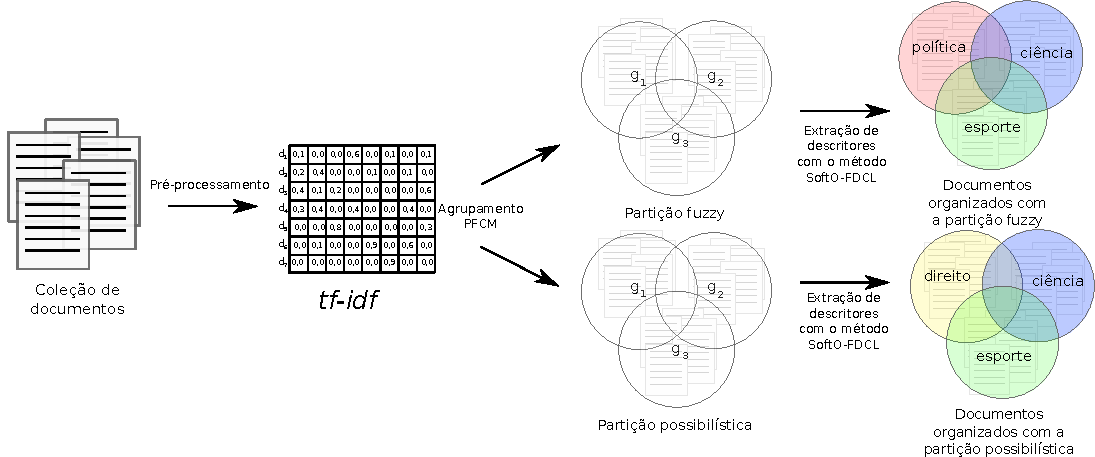
\includegraphics[width=1.0\columnwidth]{assets/process_pfcm.pdf} 
  \caption{Estratégia de organização flexível de documentos adotada ao se misturar abordagens fuzzy
  e possibilísticas no agrupamento} 
  \label{fig:flexibleorganization} 
\end{figure}

Para se calcular a quantidade ótima de grupos, para cada coleção foi utilizado o
método da silhueta fuzzy (Equação \ref{eq:fs}), método bastante utilizado com o propósito de avaliar
o agrupamento de documentos. Assim sendo, o número ideal de grupos é determinado após a execução da
silhueta fuzzy variando o número de grupos entre 2 e o número de classes de cada coleção.
Ressalta-se que em coleções que os documentos não possuem rótulos, ou seja o número de classes é
desconhecido, ainda é possível usar o método da silhueta fuzzy para definir o número ótimo de
grupos. No entanto, a quantidade máxima de grupos deve ser definida de modo empírico ou com base em
alguma informação prévia a respeito dos dados. 

Para permitir uma análise comparativa dos resultados, o experimento foi realizado também com os
algoritmos FCM e PCM.  Como resultado do agrupamento das coleções, está disposto na Tabela
\ref{table:pfcmclusters} a comparação do número de grupos obtidos por cada algoritmo de agrupamento.
Nessa comparação nota-se que os algoritmos FCM e PFCM foram os que alcançaram uma quantidade de
partições mais próxima da quantidade de classes existentes em cada coleção. Enquanto o PCM manteve
uma tendência a produzir uma quantidade menor de grupos em relação aos demais.

\begin{table}[!htp]
  \centering
  \begin{tabular}{ |l|c|c|c|c|}
    \hline
    {\bf Coleção} & {\bf \# classes} & {\bf FCM} & {\bf PCM} & {\bf PFCM} \\
    \hline
    Opinosis & 3 & 3 & 3 & 3 \\
    \hline
    20Newsgroup & 4 & 2 & 2 & 2 \\
    \hline
    Hitech & 6 & 6 & 5 & 5 \\
    \hline
    NSF & 16 & 11 & 2 & 16 \\
    \hline
    WAP & 20 & 14 & 5 & 16 \\
    \hline
    Reuters-21578 & 43 & 22 & 11 & 36 \\
    \hline
  \end{tabular}
  \caption{Quantidade ótima de grupos determinada através do método da silhueta fuzzy para cada
  algoritmo de agrupamento}
  \label{table:pfcmclusters}
\end{table}

Após agrupar os dados utilizando os métodos FCM, PCM e PFCM, foi aplicado o método de extração 
de descritores SoftO-FDCL. Para avaliar os descritores produzidos, foi verificado o
potencial preditivo dos mesmos, possibilitando assim quantificar a qualidade dos
termos selecionados para nomear os grupos. 

A avaliação do potencial preditivo dos descritores foi realizada, realizando se uma defuzificação
dos grupos produzidos pelo agrupamento, ou seja, se durante o agrupamento foi gerado o conjunto
de grupos $G = \{g_1,g_2,...,g_c\}$, temos então o conjunto de grupos $crisp$ $C' =
\{crisp_1,crisp_2,...,crisp_c\}$, onde cada $crisp_i$ corresponde ao grupo $g_i$. A função de
defuzificação adotada para se converter as
as partições fuzzy e possibilística, as quais permitem que um documento pertença a um ou mais
grupos, considera o grupo $crisp$ de um documento $d_i$, como sendo o grupo $crisp_j$ do respectivo
$grupo_j$, no qual $d_i$ possui a maior
pertinência/tipicidade. Esta definição está formalizada na Equação (\ref{eq:class}).

\begin{equation}
  crisp(d_i) = \begin{cases}
    crisp_j, & \mu(d_i,g_j) = \displaystyle\max_{\forall g \in G} \mu(d_i,g), \text{se a partição
  for fuzzy}\\
  crisp_j, & \lambda(d_i,g_j) = \displaystyle\max_{\forall g \in G} \lambda(d_i,g), \text{se a
  partição for possibilística}
  \end{cases}
  \label{eq:class}
\end{equation}

Após se atribuir os documentos aos grupos $crisp$, é produzida uma outra matriz,
considerando apenas os termos descritores dos grupos. Logo, essa matriz documentos x descritores
$D'_{n \times m}$, 
é uma versão condensada da matriz documentos x termos $D_{n \times k}$, onde $n$ corresponde a 
quantidade de documentos, $k$ à quantidade de termos e $m$ à quantidade de descritores. O conteúdo
dessa matriz condensada, assim como na matriz original, é a frequência dos descritores nos 
documentos. 

Visando avaliar a qualidade dos descritores e permitir uma comparação direta dos impactos
dessa abordagem com os resultados publicados em \citeonline{Nogueira2013} e
\citeonline{Nogueira2015}. Submeteu-se a matriz $D'$ 
aos algoritmos de classificação 
SVM, Naive Bayes, Multinomial Naive Bayes, KNN e C4.5, que são bem comuns na avaliação de 
métodos de aprendizado de máquina, e foram os mesmos utilizados em \citeonline{Nogueira2015}.

Nesse contexto, foi utilizada a implementação dos algoritmos de classificação anteriormente citados
presentes na ferramenta WEKA \cite{weka}. Os algoritmos Naive Bayes (NB), Multinomial Naive Bayes
(NB-Multinomial) e o J48 (que é a implementação do C4.5 existente no WEKA), foram executados com os
parâmetros padrão da ferramenta. Por outro lado, o SVM foi ajustado para usar o {\it Normalized
Polynomial Kernel\/} com o parâmetro de complexidade sendo $c = 2.0$. O algoritmo IBk (implementação
do KNN presente no WEKA) foi executado 7 vezes, variando o parâmetro de vizinhos de 1 até 7, sendo
escolhido o melhor resultado. Ressalta-se que foi adotada a técnica {\it 10-fold cross validation\/}
no experimento para melhor capturar a capacidade de generalização do modelo. Os resultados dessa
avaliação estão apresentados nas Figuras \ref{fig:pfcmopinosis},  \ref{fig:pfcm20news},
\ref{fig:pfcmhitech}, \ref{fig:pfcmnsf}, \ref{fig:pfcmwap} e \ref{fig:pfcmreuters}. 

\begin{figure}[!htp] \centering 
   \begin{minipage}{0.45\textwidth} 
     \centering
    \includegraphics[width=1.0\columnwidth]{assets/pfcm/opinosis} 
    \caption{Desempenho obtido com os descritores extraídos com o algoritmo SoftO-FDCL a partir dos
      métodos de agrupamento FCM,
    PCM e PFCM executados na coleção Opinosis} 
  \label{fig:pfcmopinosis}
  \end{minipage}\hfill 
  \begin{minipage}{0.45\textwidth} \centering
    \includegraphics[width=1.0\columnwidth]{assets/pfcm/newsgroup} 
    \caption{Desempenho obtido com os descritores extraídos com o algoritmo SoftO-FDCL a partir dos
      métodos de agrupamento FCM,
    PCM e PFCM executados na coleção 20Newsgroup} 
     \label{fig:pfcm20news} 
   \end{minipage} 
\end{figure}

\begin{figure}[!htp] \centering 
   \begin{minipage}{0.45\textwidth} 
     \centering
    \includegraphics[width=1.0\columnwidth]{assets/pfcm/hitech} 
    \caption{Desempenho obtido com os descritores extraídos com o algoritmo SoftO-FDCL a partir dos
      métodos de agrupamento FCM,
    PCM e PFCM executados na coleção Hitech} 
  \label{fig:pfcmhitech}
  \end{minipage}\hfill 
  \begin{minipage}{0.45\textwidth} \centering
    \includegraphics[width=1.0\columnwidth]{assets/pfcm/nsf} 
    \caption{Desempenho obtido com os descritores extraídos com o algoritmo SoftO-FDCL a partir dos
      métodos de agrupamento FCM,
    PCM e PFCM executados na coleção NSF} 
     \label{fig:pfcmnsf} 
   \end{minipage} 
\end{figure}

\begin{figure}[!htp] \centering 
   \begin{minipage}{0.45\textwidth} 
     \centering
    \includegraphics[width=1.0\columnwidth]{assets/pfcm/wap} 
    \caption{Desempenho obtido com os descritores extraídos com o algoritmo SoftO-FDCL a partir dos
      métodos de agrupamento FCM,
    PCM e PFCM executados na coleção WAP} 
    \label{fig:pfcmwap}
  \end{minipage}\hfill 
  \begin{minipage}{0.45\textwidth} \centering
    \includegraphics[width=1.0\columnwidth]{assets/pfcm/reuters} 
    \caption{Desempenho obtido com os descritores extraídos com o algoritmo SoftO-FDCL a partir dos
      métodos de agrupamento FCM,
    PCM e PFCM executados na coleção Reuters-21578} 
     \label{fig:pfcmreuters} 
   \end{minipage} 
\end{figure}

O resumo dos resultados do desempenho dos descritores extraídos após o agrupamento com os
algoritmos FCM, PCM e PFCM é apresentado na Tabela \ref{table:pfcmsummary}. Na tabela, a marcação
($\checkmark$) denota qual método de agrupamento obteve a maior taxa de classificação dentre os
demais.

\begin{table}[!htp]
  \centering
  \begin{tabular}{ |l|c c c c c c c|}
    \hline
    {\bf Coleção} & {\bf docs} & {\bf termos} & {\bf classes} & {\bf \% zeros} & {\bf FCM} & {\bf
  PCM} & {\bf PFCM} \\
    \hline
    {\bf Opinosis} & 51 & 842 & 3 & 95,73\% & & $\checkmark$ &  \\
    \hline
    {\bf 20newsgroups} & 2000 & 11028 & 4 & 99,11\% & & & $\checkmark$\\
    \hline
    {\bf Hitech} & 600 & 6925 & 6 & 97,93\% & $\checkmark$ & & \\
    \hline
    {\bf NSF} & 1600 & 2806 & 16 & 99,76\% & $\checkmark$ & & \\
    \hline
    {\bf WAP} & 1560 & 8070 & 20 & 98,51\% & & & $\checkmark$ \\
    \hline
    {\bf Reuters-21578} & 1052 & 3925 & 43 & 98,55\% & $\checkmark$ & & \\
    \hline
  \end{tabular}
  \caption{Sumário dos resultados da classificação dos descritores}
  \label{table:pfcmsummary}
\end{table}

Esses resultados obtidos reforçam a flexibilidade e adaptação do método SoftO-FDCL
\cite{Nogueira2013}, a novos algoritmos de agrupamento, demonstrando-se promissor na tarefa de
extrair termos relevantes dos grupos produzidos na etapa de agrupamento. Tal expectativa é
demonstrada por meio do potencial preditivo evidenciado na Tabela \ref{table:pfcmsummary}, com as
taxas máximas de classificação de mais de 80\% para quase todas as coleções, com exceção da base
Hitech, a qual obteve a taxa máxima de 58.67\%.  

Adicionalmente, ressalta-se a importância também de avaliar de maneira subjetiva os descritores
selecionados dos grupos, permitindo  compreender se os termos obtidos fazem sentido para a
organização de documentos em grupos. 

\begin{table}[!htp]
  \centering
  \begin{tabular}{ |l|p{4cm} | p{4cm} | p{4cm}|}
    \hline
    {\bf Método} & $crisp_1$ & $crisp_2$ & $crisp_3$ \\
    \hline
    {\bf FCM} & easy, clear, drive, display, control, car, version, nice, work, perfect & fact,
    import, isn't, model, problem, unit, design, don't, doesn't, found & breakfast, nearby,
    concierge, eat, bottle, coffee, floor, food, inn, friendly \\
    \hline
    {\bf PCM} & easy, read, problem, version, don't, small, nice, car, work, found & fact, back,
    turn, expect, size, close, quality, review, min, feature & feel, amazing, isn't, extreme, drive,
    include, point, reason, give, run\\
    \hline
    {\bf PFCM $\mu$} & easy, drive, control, don't, version, nice, car, work, perfect, lot & fact,
    isn't, read, complete, device, display, size, doesn't, found & breakfast, nearby, pleasant,
    concierge, eat, coffee, floor, clean, friendly, food\\
    \hline
    {\bf PFCM $\lambda$} & club, immaculate, send, towel, basic, exception, spotl, pillow, typical,
    fridge & pub, housekeep, holiday, tourist, tea, smoke, pm, renovate, facilite, london & usual,
    central, forum, bottle, modern, adult, supply, food, reserve, dinner\\
    \hline
  \end{tabular}
  \caption{Descritores extraídos com os métodos de agrupamento FCM, PCM e PFCM da coleção Opinosis,
  onde $\mu$ e $\lambda$ se referem as partições fuzzy e possibilística respectivamente, da qual os
descritores foram extraídos.}
  \label{table:pfcmdescriptors}
\end{table}

Sendo assim, para uma análise subjetiva dos resultados, os descritores da coleção Opinosis, foram
obtidos por possuir poucos grupos e assim facilitar a análise e a visualização. A coleção Opinosis
contém opiniões dos usuários a respeito de serviços de hospedagem, dispositivos eletrônicos e carros
e espera-se que os descritores de grupos se aproximem semanticamente de tais categorias.  Na Tabela
\ref{table:pfcmdescriptors} tem-se a seleção de descritores escolhidos para cada grupo, extraídos
pelos algoritmos FCM, PCM e PFCM. Ao analisar os descritores selecionados é possível notar uma
tendência geral, do grupo $crisp_1$ conter descritores relacionadas a carros, o $crisp_2$ conter
descritores sobre dispositivos eletrônicos e o grupo $crisp_3$ descritores sobre hospedagem e
alimentação. Contudo, nota-se que os descritores do PCM e do PFCM$\lambda$ (descritores da partição
possibilística do PFCM) estão um pouco mais misturados, não apresentando uma tendência geral bem
definida. Uma explicação possível a esse resultado pode se encontrar na própria partição
possibilística a qual permite que um mesmo documento possua um grau de tipicidade elevado em todos
os grupos. Neste contexto, uma solução possível pode ser uma adaptação do método de extração de
descritores SoftO-FDCL voltado para a partição possibilística, assim como também para algoritmos
híbridos com duas partições, que é o caso do PFCM.

De maneira complementar, é importante salientar que o método de extração de descritores SoftO-FDCL é
totalmente influenciado pelos valores contidos nas partições fuzzy e possibilística. Portanto, é
também importante realizar uma análise dos métodos de agrupamento utilizados nos experimentos, com
a finalidade de entender qual método é mais apropriado em determinados contextos. Os resultados apontam que a dimensionalidade das bases foi um fator determinante no desempenho dos
métodos de agrupamento para a organização flexível de documentos, e, consequentemente, a
extração de descritores. Por exemplo, do sumário de resultados apresentados na Tabela
\ref{table:pfcmsummary}, é possível observar que o método PCM obteve o melhor resultado na coleção
Opinosis, que possui a menor dimensionalidade (842 termos), enquanto que o algoritmo FCM superou os
demais métodos na coleção NSF (2806 termos), Reuters-21578 (3925 termos), Hitech (6925 termos), e por
fim o algoritmo PFCM atingiu melhores resultados para as coleções WAP (8070 termos) e 20Newsgroup
(11028 termos), que são as coleções de maior dimensionalidade.

Na próxima seção, motivado pelos resultados desses experimentos será explorado, uma adaptação do
método SoftO-FDCL para evitar o processo de extração dupla de descritores em algoritmos que possuam
partições fuzzy e possibilística.

\section{Uma abordagem híbrida para extração de descritores}

Nos experimentos anteriores foi identificado um possível problema ao realizar a extração dos
descritores de maneira separada em cada partição do PFCM, assim como também foi apontado que o
método pode não capturar toda essência da partição possibilística, que difere da partição fuzzy do
FCM por não possuir a restrição que obriga a soma das pertinências de um grupo ser igual a um
(Equação \ref{eq:fcmrestri1}).
Logo, é intuitivo indagar que para uma melhor interpretação dos grupos produzidos em um método de
agrupamento híbrido, seja pertinente utilizar também uma abordagem mista de extração de descritores.
Aproveitando-se assim dos benefícios existentes na partição possibilística, a qual penaliza os
elementos ruidosos, com baixos valores de tipicidade, sem abrir mão das vantagens presentes na
partição fuzzy. Para isso é necessário compreender os mecanismos de funcionamento do método
SoftO-FDCL, para que seja possível propor uma adaptação para este contexto.

\subsection{Investigações na extração de descritores em partições possibilísticas}
\label{sec:softofdcl}

O método SoftO-FDCL ({\it Soft Organization - Fuzzy Description Comes Last}) proposto em 
\citeonline{Nogueira2013} é baseado em uma adaptação das medidas clássicas de Recuperação de
Informação (RI), para quantificar a relevância dos termos candidatos à descritores dos grupos
obtidos na etapa de agrupamento, utilizando a informação de pertinência ou tipicidade advinda do
algoritmo de agrupamento.  Esse grau de compatibilidade entre um documento e um grupo, desempenha um
papel fundamental na seleção dos termos candidatos a descritores de um determinado grupo, pois
através deste, é possível penalizar os termos de documentos que possuam baixo grau de
compatibilidade com o grupo no qual o descritor está sendo extraído.  

Para realizar a extração dos descritores, inicialmente todos os termos que permanecem na coleção
após a etapa de pré-processamento são considerados como candidatos a descritores. Posteriormente o
método realiza uma avaliação quantitativa da relevância de cada termo $t_k$ para um grupo $g_j$,
utilizando a medida $f1$ apresentada na Equação \ref{eq:fmeasure}, que é a média harmônica da
precisão (Equação \ref{eq:precision}) e da revocação (Equação \ref{eq:recall}).  A medida de
precisão checa a quantidade de documentos significantes entre os documentos recuperados. Enquanto a
medida de revocação calcula a proporção de documentos relevantes recuperados entre todos os
documentos relevantes da coleção. Tanto a medida de precisão quanto a de revocação, tomam como base
as informações obtidas a partir da matriz de contingência apresentada na Tabela
\ref{table:softmatrix}. Adicionalmente tem-se que um documento $d_i$ é considerado como parte do
grupo $g_j$, caso $\mu(d_j,g_j) \geq \delta$ para valores de pertinências ou $\lambda(d_i,g_j) \geq
\delta$ para partição possibilística, onde $\delta = \frac{1}{c}$ e $c$ a quantidade de grupos. O
limiar $\delta$ é uma parte relevante do método SoftO-FDCL, pois ele possibilita considerar como
candidatos a descritores, os termos presentes em documentos que pertençam a mais de um grupo, ao
mesmo tempo que também penaliza os termos presentes em documentos com baixa compatibilidade em um
grupo.

\begin{table}[!htp]
  \centering
  \begin{tabular}{ |p{5cm}|p{5cm}|p{5cm}|}
    \cline{2-3}
    \multicolumn{1}{p{5cm}|}{} & Documentos do grupo $g_j$ com grau de compatibilidade 
    maior ou igual a $\delta$ &
    Documentos do grupo $g_j$ com grau de compatibilidade menor do que $\delta$ \\
    \hline
    Documentos que possuem o descritor candidato $t_k$ & \parbox[c]{5cm}{\centering $ganhos$} &
    \parbox[c]{5cm}{\centering \it ruídos\/} \\
    \hline
    Documentos que não possuem o descritor candidato $t_k$ & \parbox[c]{5cm}{\centering $perdas$} &
    \parbox[c]{5cm}{\centering $rejeitos$} \\
    \hline
  \end{tabular}
  \caption{Matriz de contingência do termo $t_k$ para o grupo $g_j$ para as medidas de recuperação
  de informação}
  \label{table:softmatrix}
\end{table}

\begin{equation}
  precis\tilde{a}o(t_k,g_j) = \frac{ganhos}{ganhos + \text{\it ruídos}}
  \label{eq:precision}
\end{equation}
\begin{equation}
  \text{\it recuperação\/}(t_k,g_j) = \frac{ganhos}{ganhos + perdas}
  \label{eq:recall}
\end{equation}
\begin{equation}
  f1(t_k,g_j) = \frac{2 * \text{\it precisão}(t_k,g_j) * \text{\it recuperação}(t_k,g_j)}
  {\text{\it precisão}(t_k,g_j) + \text{\it recuperação}(t_k,g_j)}
  \label{eq:fmeasure}
\end{equation}

Para efetuar a seleção dos termos descritores, é construído um $ranking$ dos termos candidatos de
cada grupo, ordenados pela pontuação obtida com a medida $f1$ (Equação \ref{eq:fmeasure}). A partir
dessa pontuação, os termos com as maiores pontuações em cada grupo são selecionados.
\citeonline{Nogueira2013} destaca que a quantidade de descritores a ser selecionada fica a critério
do usuário.

Em síntese, o método SoftO-FDCL cria uma tabela de pontuação dos termos candidatos aos grupos,
e seleciona os que obtiverem melhores valores de $f1$.  

Formalizando essa
percepção, é possível definir as duas propriedades que derivam dessa discussão, as quais são as
Equações (\ref{eq:limiarp1}) e (\ref{eq:limiarp2}). A primeira
propriedade  apresentada na Equação (\ref{eq:limiarp1}) expressa que se um documento possuir pertinência maior do
que o limiar $\delta$ em um grupo $g_1$ qualquer, obrigatoriamente existirá ao menos um outro grupo
$g_2$ no qual esse mesmo documento terá pertinência inferior ao limiar $\delta$. Portanto, essa
propriedade nos indica que na maioria das vezes um ou mais documentos serão descartados na análise
dos termos candidatos do grupo, o que reforça a adequação desse limiar para a partição de
pertinências. Por outro lado, a segunda
propriedade apresentada na Equação (\ref{eq:limiarp2}) denota o único caso particular, no qual um documento $d_i$
não será descartado em nenhum grupo. Isto ocorre apenas se $d_i$ possuir pertinência igual ao limiar em todos
os grupos, o que só acontece em dados ruidosos, que apresentam o problema do elemento equidistante
detalhado na Figura \ref{fig:fcm_problem} do Capítulo 2.

\begin{equation}
  \mu(d_1,g_1) > \delta \rightarrow \exists \mu(d_i, g_2) < \delta
  \label{eq:limiarp1}
\end{equation}
\begin{equation}
  ( \mu(d_1,g_1) = \delta ) \wedge ( \mu(d_i,g_2) = \delta ) \wedge ... \wedge ( \mu(d_i,g_{c-1}) =
  \delta ) \rightarrow ( \mu(d_i, g_c) = \delta  )
  \label{eq:limiarp2}
\end{equation}

Contudo, para a partição possibilística, essas duas propriedades não são satisfeitas. Isso ocorre
devido a remoção da restrição da Equação (\ref{eq:fcmrestri1}), o que permite o grau de
compatibilidade da partição possibilística variar de maneira independente entre o intervalo de
$[0,1]$, sem ser influenciado pelo grau de compatibilidade do documento nos demais grupos.

Para tornar claro essas análises, considere uma situação onde tem-se uma coleção de textos com
3 documentos (Tabela \ref{table:sampledocuments}), onde cada documento possui 3 termos. Essa coleção
de documentos foi agrupada, usando o método PFCM, o qual produziu 2 grupos, com as suas
respectivas partições de pertinência (Tabela
\ref{table:samplefcmclusters}) e possibilística (Tabela \ref{table:samplepcmclusters}).

\begin{table}[!htp]
  \centering
  \begin{tabular}{ |c|c|c|c|}
    \hline
    & $\mathbfit{t_1}$ & $\mathbfit{t_2}$ & $\mathbfit{t_3}$ \\
    \hline
    $\mathbfit{d_1}$ & 0 & 0 & 1 \\
    \hline
    $\mathbfit{d_2}$ & 1 & 1 & 0 \\
    \hline
    $\mathbfit{d_2}$ & 1 & 1 & 0 \\
    \hline
  \end{tabular}
  \caption{Exemplo de matriz documentos x termos}
  \label{table:sampledocuments}
\end{table}

\begin{table}[!htp]
  \begin{minipage}{0.45\textwidth} 
    \centering
    \begin{tabular}{ |c|c|c|}
      \hline
      & $\mathbfit{g_1}$ & $\mathbfit{g_2}$ \\
      \hline
      $\mathbfit{d_1}$ & 0.5 & 0.5 \\
      \hline
      $\mathbfit{d_2}$ & 0.3 & 0.7 \\
      \hline
      $\mathbfit{d_3}$ & 0.3 & 0.7 \\
      \hline
    \end{tabular}
    \caption{Exemplo de matriz documents x grupos com graus de pertinência}
    \label{table:samplefcmclusters}
  \end{minipage}\hfill 
  \begin{minipage}{0.45\textwidth} 
    \centering
    \begin{tabular}{ |c|c|c|}
      \hline
      & $\mathbfit{g_1}$ & $\mathbfit{g_2}$ \\
      \hline
      $\mathbfit{d_1}$ & 0.7 & 0.7 \\
      \hline
      $\mathbfit{d_2}$ & 0.5 & 0.8 \\
      \hline
      $\mathbfit{d_3}$ & 0.5 & 0.9 \\
      \hline
    \end{tabular}
    \caption{Exemplo de matriz documents x grupos com graus de possibilidade}
    \label{table:samplepcmclusters}
  \end{minipage}\hfill 
\end{table}

A partir desse agrupamento é possível aplicar a extração de descritores, utilizando as partições
apresentadas nas Tabelas \ref{table:samplefcmclusters} e \ref{table:samplepcmclusters}. Seguindo
o procedimento do método SoftO-FDCL, inicialmente devemos considerar todos os descritores
presentes na Tabela \ref{table:sampledocuments}, como candidatos a descritores. Então, para
promover os descritores candidatos do grupo $g_1$ utilizando os graus de pertinências, deve-se 
observar os documentos que possuem pertinência maior ou igual ao limiar, onde no exemplo é
igual a $\delta = \frac{1}{2} = 0.5$. Portanto, o único documento que se enquadra no filtro do limiar
é o documento $d_1$ e o termo $t_3$, que é o único presente no documento $d_1$, é promovido
a descritor candidato e consequentemente a descritor do grupo $g_1$. Já o grupo $g_2$ possui 3
documentos com pertinência maior ou igual ao limiar $\delta$. Sendo assim, os termos de $d_1,d_2$ e
$d_3$ são promovidas a descritores candidatos do grupo $g_2$. Ao calcular-se a medida $f1$ para cada
um deles temos: $f1(t_1,g_2) = 0,8$, $f1(t_2,g_2) = 0,8$, $f1(t_3,g_2) = 0,5$. Logo, os descritores
selecionados para cada grupo foram $g_1 =\{t_3\}$ e $g_2 = \{t_1, t_2\}$.

Ao aplicar a extração de descritores sobre a partição possibilística, tem-se agora
os documentos $d_1, d_2$ e $d_3$ considerados parte do grupo $g_1$, de acordo com a regra do
limiar. Logo, deve-se considerar os termos dos 3 documentos como descritores candidatos. Os valores
de $f1$ para os 3 termos candidatos do grupo $g_1$ são: $f1(t_1,g_1) = 0,8$,
$f1(t_2,g_1) = 0,8$, $f1(t_3,g_1) = 0,5$. Para o grupo $g_2$ obtém-se os mesmos termos
candidatos, pois $d_1, d_2$ e $d_3$ também possuem valores de tipicidade maiores ou igual ao limiar
$\delta$, portanto os valores de $f1$ para o grupo $g_2$ são:  $g_1$: $f1(t_1,g_1) = 0,8$,
$f1(t_2,g_1) = 0,8$, $f1(t_3,g_2) = 0,5$. Foi obtido a mesma pontuação para os mesmos termos
candidatos nos dois grupos. Com isso, fica claro as causas que levaram a extração dos descritores
confusos apresentados na Tabela \ref{table:pfcmdescriptors}.  Ao se utilizar a mesma intepretação
dos graus de pertinência do FCM, nas tipicidades, o critério chave de descarte dos documentos de
baixa relevância em um grupo deixou de fazer efeito.

É importante ressaltar que esta situação se agrava ainda mais com o aumento do número de grupos
produzidos pelo agrupamento, pois quanto maior for a quantidade de grupos, menor será o valor do
limiar $\delta$. Esta noção fica explícita na terceira propriedade do limiar apresentada na Equação
(\ref{eq:limiarp3}). Ou seja, mais facilmente os graus de compatibilidade possibilísticos irão
passar no filtro do limiar, e, consequentemente todos os documentos serão considerados relevantes
para todos os grupos. 

\begin{equation}
  \lim_{c \rightarrow \infty} \delta = 0
  \label{eq:limiarp3}
\end{equation}


Na próxima seção será descrito uma possível proposta para interpretação dos graus de compatibilidade
das partições possibilística.

\subsection{Interpretando os graus de compatibilidade das partições possibilísticas}

A interpretação direta dos graus de compatibilidade possibilísticos gera uma série de problemas na
extração de descritores, conforme ficou demonstrado na seção anterior. Com isso, podemos formular a
seguinte pergunta: Como interpretar corretamente os graus de compatibilidade possibilísticos para
corretamente identificar os documentos relevantes de um dado grupo? Sabe-se que o valor de
tipicidade pode variar livremente entre o intervalo $[0,1]$, sem a restrição probabilística
(Equação \ref{eq:fcmrestri1}) do FCM. Essa é uma
característica positiva introduzida em \citeonline{Krishnapuram1993}, a qual atribui valores de
pertinência mais justos aos grupos fuzzy, em consonância com a teoria de conjuntos fuzzy proposta em
\citeonline{Zadeh1965} e brevemente contextualizada no Capítulo 2. Para melhor compreendermos esse
conceito de valores mais justos, podemos analisar o que os autores defenderam na publicação
original:

\begin{citacao}
Since our membership functions correspond more closely to
the notion of typicality, the resulting algorithms are naturally
more immune to noise. Noise points will have low degrees
of compatibility in all clusters, which makes their effect on
the clustering negligible \cite{Krishnapuram1993}.
\end{citacao}
Portanto, a vantagem em deixar os graus de compatibilidade independentes é a de se expressar a
relevância/importância real de um elemento em relação a um grupo, o que consequentemente torna o
método mais robusto e menos suscetível a ruídos. Para identificar a importância de um
documento em um grupo, pode-se por exemplo escolher em qual grupo um documento $d_i$ deveria ser
considerado relevante, considerando o grupo em que esse documento $d_i$ possuísse o maior grau de
compatibilidade. No entanto, essa estratégia resultaria em uma extração de descritores $crisp$,
perdendo assim toda a flexibilidade proporcionada nas partições $soft$ \cite{Nogueira2013}.

Sendo assim, é necessária uma estratégia que consiga interpretar bem os graus de compatibilidade,
de modo a se conservar a flexibilidade inerente à partição fuzzy, sem sacrificar a robustez contra
ruídos da tipicidade. 

Nesse contexto, propõe-se realizar tal interpretação em duas etapas. A primeira será constituída de
uma conversão da tipicidade oriunda do PCM para a pertinência do FCM, de maneira a se satisfazer a
restrição probabilística do FCM (Equação \ref{eq:fcmrestri1}). No entanto, ao apenas realizar a
conversão perde-se a robustez contra ruídos do PCM. Por isso, é possível contornar essa situação
adicionando uma penalidade ao cálculo da pontuação dos termos.

A conversão proposta dos valores de tipicidade para pertinência, dar-se a como apresentado na
Equação (\ref{eq:tip2pert}), a qual satisfaz a condição necessária (Equação
\ref{eq:tiplinharestri1}) para que o limiar $\delta$ seja aplicado, sem sofrer o problema de
considerar um documento como relevante em todos os grupos.

\begin{equation}
  \lambda'(d_i,g_j) = \frac{\lambda(d_i,g_j)}{\sum_{k=1}^c \lambda(d_i,g_k)}
  \label{eq:tip2pert}
\end{equation}

\begin{equation}
  \sum_{k=1}^c \lambda'(d_i,g_k) = 1
  \label{eq:tiplinharestri1}
\end{equation}

Entretanto, apenas realizar a conversão não atende aos dois requisitos exigidos. Para isso
vamos adaptar a matriz de contingência apresentada na Tabela \ref{table:softmatrix}, adicionando uma
ponderação as medidas, de modo a adicionar uma gratificação nos termos de documentos com elevada
tipicidade e penalizar os termos de documentos com baixo valor de tipicidade, uma estratégia de
ponderação similar é encontrada no método SoftO-wFDCL ({\it Soft Organization - weighted Fuzzy
Description Comes Last}) em \citeonline{Nogueira2013}, porém esse método, assim como o SoftO-FDCL
não se propõem a interpretar as tipicidades da partição possibilística de maneira diferenciada.

A adaptação sugerida da matriz de contingência está apresentada na Tabela \ref{table:softmatrix2},
na qual os valores de ganhos, perdas, ruídos e rejeitos foram mapeados para as Equações
(\ref{eq:ganhos}), (\ref{eq:perdas}),  (\ref{eq:ruidos}) e  (\ref{eq:rejeitos}) respectivamente.
Portanto ao invés de realizar uma contagem discreta dos ganhos, perdas, ruídos e rejeitos, é
realizado uma soma contínua das contribuições de cada documento ao grupo, considerando o valor de
tipicidade. Desse modo, conseguimos reduzir a contribuição de documentos com baixa tipicidade no
grupo e aumentar a contribuição de documentos com alta tipicidade no grupo. Resultando assim, em uma
pontuação mais justa e mais coerente dos termos extraídos dos grupos. Os ajustes necessários nas
medidas de precisão e recuperação estão detalhados nas equações (\ref{eq:precision2}) e
(\ref{eq:recall2}), enquanto o cálculo da medida $f1(t_k,g_j)$ permanece como definido na Equação
(\ref{eq:fmeasure}). Destaca-se que nestas equações o limiar $\delta$ passa a ser verificado com os
valores de tipicidades convertidos, ilustrados pela função $\lambda'(d_i,g_j)$ (Equação
\ref{eq:tip2pert}) e $\varphi(t_i,d)$ refere-se a frequência do termo $t_i$ no documento $d$, de
acordo com a Equação (\ref{eq:tfidf}).

\begin{table}[!htp]
  \centering
  \begin{tabular}{ |p{5cm}|p{5cm}|p{5cm}|}
    \cline{2-3}
    \multicolumn{1}{p{5cm}|}{} & Documentos do grupo $g_j$ com grau de compatibilidade 
    maior ou igual a $\delta$ &
    Documentos do grupo $g_j$ com grau de compatibilidade menor do que $\delta$ \\
    \hline
    Documentos que possuem o descritor candidato $t_k$ & \parbox[c]{5cm}{\centering
  $ganhos(t_k,g_j)$} & \parbox[c]{5cm}{\centering \it ruídos\/$(t_k,g_j)$} \\
    \hline
    Documentos que não possuem o descritor candidato $t_k$ & \parbox[c]{5cm}{\centering
  $perdas(t_k,g_j)$} & \parbox[c]{5cm}{\centering $rejeitos(t_k,g_j)$} \\
    \hline
  \end{tabular}
  \caption{Matriz de contingência do termo $t_k$ para o grupo $g_j$ adaptada para a partição
  possibilística}
  \label{table:softmatrix2}
\end{table}

\begin{equation}
  ganhos(t_i,g_j) = 
  \sum_{
      d \in D' 
  } \lambda(d,g_j), D' = \left\{d | d \in D, \lambda'(d,g_j) \geq \delta, \varphi(t_i,d) > 0
  \right\}
  \label{eq:ganhos}
\end{equation}
\begin{equation}
  perdas(t_i,g_j) = 
  \sum_{
      d \in D' 
  } \lambda(d,g_j), D' = \left\{d | d \in D, \lambda'(d,g_j) \geq \delta, \varphi(t_i,d) = 0
  \right\}
  \label{eq:perdas}
\end{equation}
\begin{equation}
  \text{\it ruídos\/}(t_i,g_j) = 
  \sum_{
      d \in D' 
  } \lambda(d,g_j), D' = \left\{d | d \in D, \lambda'(d,g_j) < \delta, \varphi(t_i,d) > 0 \right\}
  \label{eq:ruidos}
\end{equation}
\begin{equation}
  \text{\it rejeitos\/}(t_i,g_j) = 
  \sum_{
      d \in D' 
  } \lambda(d,g_j), D' = \left\{d | d \in D, \lambda'(d,g_j) < \delta, \varphi(t_i,d) = 0 \right\}
  \label{eq:rejeitos}
\end{equation}

\begin{equation}
  precis\tilde{a}o(t_k,g_j) = \frac{ganhos(t_k,g_j)}{ganhos(t_k,g_j) + \text{\it ruídos}(t_k,g_j)}
  \label{eq:precision2}
\end{equation}
\begin{equation}
  \text{\it recuperação\/}(t_k,g_j) = \frac{ganhos(t_k,g_j)}{ganhos(t_k,g_j) + perdas(t_k,g_j)}
  \label{eq:recall2}
\end{equation}

Nas próximas duas seções as duas abordagens que derivam dessa interpretação são descritas. A
primeira, é uma proposta de extensão do método SoftO-FDCL voltado para a partição possibilística do
PCM, com a interpretação apresentada nessa sessão. Enquanto a segunda abordagem, apresenta uma
estratégia de extração de descritores para o algoritmo PFCM, interpretando em conjunto as duas
partições presentes no algoritmo.

\subsection{O método PDCL}

A agora que a proposta de interpretação da partição possibilística está concluída, 
o método para extração de descritores para a partição possibilística, o qual
será denominado aqui de PDCL ({\it Possibilistic Descriptor Comes Last\/}) é proposto. Para realizar a extração
de descritores, o método PDCL considera inicialmente todos os termos como candidatos. Em seguida,
para cada grupo $g_j$ a precisão (Equação \ref{eq:precision2}) e recuperação (Equação
\ref{eq:recall2}) de todos os termos $t_k$ são calculados. A partir destes valores, a
pontuação de cada termo $t_k$ no grupo $g_j$ é calculada, utilizando-se a medida $f1(t_k,g_j)$ (Equação
\ref{eq:fmeasure}). A partir dessa pontuação por grupo dos termos candidatos, deve-se selecionar
os $m$ descritores de maior pontuação em cada grupo. A quantidade $m$ de descritores é
definida pelo usuário. Um detalhamento do método PDCL está apresentado no Algoritmo \ref{alg:pdcl}.

\subsection{O método Mixed-PFDCL}

Na discussão do experimento da seção \ref{sec:exppfcm}, onde foram apresentados os resultados do
refinamento com o método PFCM ({\it Possibilistic Fuzzy C Means\/}) na proposta de organização
flexível de documentos, foi salientado, a importância de uma estratégia que conseguisse
capturar a filosofia híbrida do algoritmo PFCM, levando em consideração suas duas partições. 

Uma das características presentes no método PFCM, é a adição dos parâmetros $a$ e $b$ que atuam como
reguladores da influência do FCM e do PCM no agrupamento obtido. Portanto, é importante destacar a
relevância de tais parâmetros no processo de extração de descritores, objetivando
assim mais coerência com o algoritmo e exatidão nos resultados..

Nesse contexto, é também proposta a combinação dos valores de pertinência e de tipicidade
convertendo-os em um único grau de compatibilidade conforme Equação (\ref{eq:pfcmmix}). Essa
combinação refere-se à média ponderada dos valores de pertinência e tipicidade pelos parâmetros $a$
e $b$ do método PFCM.

\begin{equation}
  \mu'(d_i,g_j) = \frac{a \mu(d_i,g_j) + b \lambda'(d_i,g_j)}{a+b}
  \label{eq:pfcmmix}
\end{equation}

Como resultado dessa combinação, a estratégia definida anteriormente na Figura
\ref{fig:flexibleorganization} é alterada, eliminando a dupla extração de descritores do método
SoftO-FDCL do agrupamento produzido por meio do PFCM, na abordagem híbrida de extração de
descritores com o método Mixed-PFDCL proposto. Essa nova estratégia proposta está contextualizada na
Figura \ref{fig:pfdclprocess}.

\begin{figure}[!htp] 
  \centering
  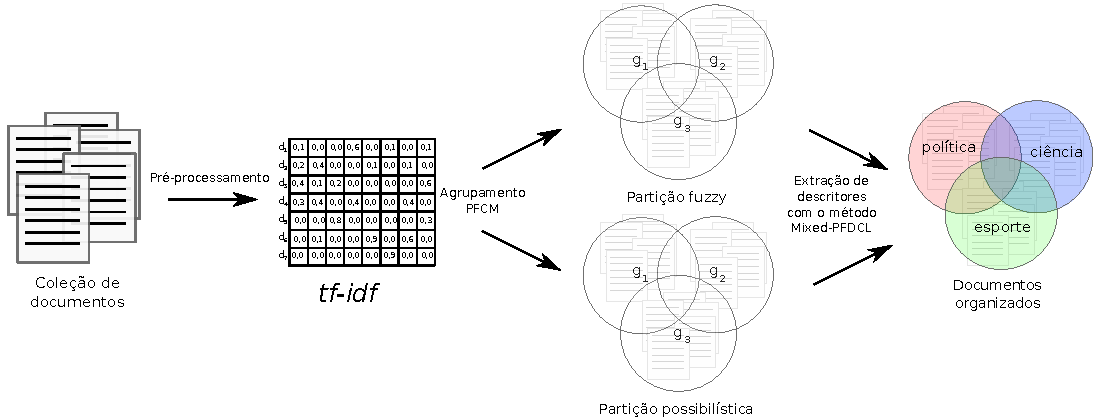
\includegraphics[width=1.0\columnwidth]{assets/process_pfdcl.pdf} 
  \caption{Estratégia híbrida proposta para uma organização flexível de documentos com o 
  agrupamento com o método PFCM e a extração de descritores com o método Mixed-PFDCL.} 
  \label{fig:pfdclprocess} 
\end{figure}


Como resultado dessa combinação é preciso adaptar as medidas de ganhos, perdas, ruídos e rejeitos,
de forma a considerar a relevância de um dado documento $d$ em relação ao limiar $\delta$, a partir
da pertinência híbrida $\mu'(d_i,g_j)$. 

Essa adaptação está então disposta nas Equações (\ref{eq:ganhos2}), (\ref{eq:perdas2}),
(\ref{eq:ruidos2}) e (\ref{eq:rejeitos2}). Ressalta-se que foi mantido no somatório de ganhos,
perdas, ruídos e rejeitos, o valor de tipicidade, devido a capacidade do mesmo em expressar a real
relação de pertinência de um documento a um grupo, devido a remoção da restrição probabilística
(Equação \ref{eq:fcmrestri1}) do
FCM. As demais medidas de precisão, recuperação e $f1$, permanecem com a mesma
definição apresentada anteriormente. Para uma melhor compreensão do método proposto, um pseudo
código do método Mixed-PFDCL está apresentado no Algoritmo \ref{alg:mixedpfdcl}.

\begin{equation}
  ganhos(t_i,g_j) = 
  \sum_{
      d \in D' 
  } \lambda(d,g_j), D' = \left\{d | d \in D, \mu'(d,g_j) \geq \delta, \varphi(t_i,d) > 0
  \right\}
  \label{eq:ganhos2}
\end{equation}
\begin{equation}
  perdas(t_i,g_j) = 
  \sum_{
      d \in D' 
  } \lambda(d,g_j), D' = \left\{d | d \in D, \mu'(d,g_j) \geq \delta, \varphi(t_i,d) = 0
  \right\}
  \label{eq:perdas2}
\end{equation}
\begin{equation}
  \text{\it ruídos\/}(t_i,g_j) = 
  \sum_{
      d \in D' 
  } \lambda(d,g_j), D' = \left\{d | d \in D, \mu'(d,g_j) < \delta, \varphi(t_i,d) > 0 \right\}
  \label{eq:ruidos2}
\end{equation}
\begin{equation}
  \text{\it rejeitos\/}(t_i,g_j) = 
  \sum_{
      d \in D' 
  } \lambda(d,g_j), D' = \left\{d | d \in D, \mu'(d,g_j) < \delta, \varphi(t_i,d) = 0 \right\}
  \label{eq:rejeitos2}
\end{equation}

\begin{algorithm}[!htp] 
  \SetAlgoLined 
  \textbf{{\color{blue}pdcl}(P, D, G, m)}\\
  \Begin{
    descritores $\gets \emptyset$\;
    \ForEach{$g \in G$}{
      candidatos $\gets [t_1,t_2,...,t_k]$\;
      ranking $\gets \emptyset$\;
      \ForEach{$t \in$ candidatos}{
        precisao $\gets$ Equação (\ref{eq:precision})\;
        recuperacao $\gets$ Equação (\ref{eq:recall})\;
        pontuacao $\gets$ Equação (\ref{eq:fmeasure})\;
        ranking[t] $\gets$ pontuacao\;
      }
      descritores[g] $\gets$ $m$ termos do ranking com maior pontuacao\;
    }
    $\textbf{retorne}$ (descritores)\; 
  }
  \caption{Pseudo código do método de extração de descritores PDCL. Onde
    considere P a partição
  possibilística (Equação \ref{eq:pcmpart}), D a coleção de documentos da coleção, G os grupos
produzidos pelo método de agrupamento e $m$ a quantidade descritores desejada por grupo.}
\label{alg:pdcl} 
\end{algorithm}

\begin{algorithm}[!htp] 
  \SetAlgoLined 
  \textbf{{\color{blue}mixed-pfdcl}(U, P, D, G, m, a, b)}\\
  \Begin{
    descritores $\gets \emptyset$\;
    \ForEach{$g \in G$}{
      candidatos $\gets [t_1,t_2,...,t_k]$\;
      ranking $\gets \emptyset$\;
      \ForEach{$t \in$ candidatos}{
        precisao $\gets$ Equação (\ref{eq:precision2})\;
        recuperacao $\gets$ Equação (\ref{eq:recall2}) \;
        pontuacao $\gets$ Equação (\ref{eq:fmeasure})\;
        ranking[t] $\gets$ pontuacao\;
      }
      descritores[g] $\gets$ $m$ termos do ranking com maior pontuacao\;
    }
    $\textbf{retorne}$ (descritores)\; 
  }
  \caption{Pseudo código do método de extração de descritores Mixed-PFDCL. Onde
    considere U a
  partição de pertinências fuzzy (Equação \ref{eq:part_fuzzy}), P a partição
  possibilística (Equação \ref{eq:pcmpart}), D a coleção de documentos da coleção, G os grupos
produzidos pelo método de agrupamento, $m$ a quantidade descritores desejada por grupo e $a,b$ os
parâmetros do PFCM.}
\label{alg:mixedpfdcl} 
\end{algorithm}

\subsection{Resultados}

Para mensurar os impactos das duas propostas (PDCL e Mixed-PFDCL) para extração de descritores apresentadas
aqui nesta seção, foi realizado outro experimento, com os algoritmos PCM e PFCM, com as bases
apresentadas na seção \ref{section:datasets}. Durante o experimento fora utilizado os métodos de
extração de descritores SoftO-FDCL, PDCL, Mixed-PFDCL. 

Uma vez que as propostas aqui apresentadas têm por objetivo otimizar os resultados apresentados
anteriormente, foi adotada uma metodologia similar aos experimentos anteriores. Ou seja, o agrupamento
final obtido para cada base, é resultado dos grupos que obtiveram o maior valor na medida de
silhueta fuzzy. Onde a quantidade de grupos para cada base, variou entre 2 e o número de classes
de cada base (Tabela \ref{table:datasets}). Ressalta-se ainda que para minimizar os efeitos da
aleatoriedade da partição inicial nesse experimento, o agrupamento foi executado 5 vezes para cada
quantidade de grupos na silhueta fuzzy. 

Os parâmetros $m$ e $n$ que regulam a variação entre fuzzy e $crisp$ das partições resultantes,
conforme ilustrados nas Figuras \ref{fig:cluster_crisp} e \ref{fig:cluster_fuzzy} foram definidos
para 1,2 de maneira empírica. De maneira geral, observou-se que as bases de maior dimensionalidade,
estavam produzindo grupos coincidentes mais facilmente, quando os valores de $m$ e $n$ eram maior do
que $1.5$. Por sua vez, os parâmetros $a$ e $b$ do algoritmo PFCM, o qual define a influência das
pertinências fuzzy do FCM e os graus de compatibilidade possibilísticos do PCM respectivamente,
foram definidos como sendo $a = 1,0$ e $b = 1,2$. Essa escolha deriva das conclusões apresentadas
em \citeonline{Pal2005}, o qual sugere que de acordo com a função objetivo (Equação
\ref{eq:pfcmobj}) do PFCM, se forem utilizados valores de $a$ maiores que $b$, os protótipos dos grupos
são mais influenciados pelas pertinências. Contudo, como em coleções textuais 
naturalmente esparsas é mais comum haver documentos ruidosos, o qual não se encaixe totalmente em
nenhum grupo, foi adotado o valor de $b$ maior do que $a$, para reduzir os efeitos
indesejados dos ruídos.

As coleções foram então agrupadas com os métodos PCM e PFCM, utilizando a metodologia descrita. A
quantidade ótima de grupos, obtida com o método da silhueta fuzzy, está apresentado na Tabela
\ref{table:pfcmclusters}. Os resultados apresentado nesta tabela, reforçam as conclusões
apresentadas experimento anterior, de que a quantidade de grupos ótima do método PFCM tende a se
aproximar mais da quantidade original de classes de cada coleção, enquanto o método PCM possui uma
tendência em obter um número de grupos bem inferior a quantidade original de classes.

\begin{table}[!htp]
  \centering
  \begin{tabular}{ |l|c|c|c|c|}
    \hline
    {\bf Coleção} & {\bf \# classes} & {\bf PCM} & {\bf PFCM} \\
    \hline
    Opinosis & 3 & 2 & 3 \\
    \hline
    20Newsgroup & 4 & 4 & 4 \\
    \hline
    Hitech & 6 & 2 & 6 \\
    \hline
    NSF & 16 &  2 & 8 \\
    \hline
    WAP & 20 & 2 & 17 \\
    \hline
    Reuters-21578 & 43 & 4 & 40 \\
    \hline
  \end{tabular}
  \caption{Quantidade ótima de grupos determinada através do método da silhueta fuzzy para cada
  algoritmo de agrupamento no segundo experimento conduzido com os métodos PCM e PFCM}
  \label{table:pfcmclusters}
\end{table}

Em seguida, foi realizado a extração dos descritores sobre as partições ótimas encontradas por
cada algoritmo de agrupamento, sobre as coleções textuais. Como a motivação desse experimento, foi
avaliar a qualidade dos descritores produzidos pelos métodos PDCL e Mixed-PFDCL propostos, a extração
de descritores foi também realizada com o método SoftO-FDCL, possibilitando assim compararmos os
resultados. E assim como no experimento anterior, essa análise quantitativa dos descritores
produzidos, foi feita, utilizando a mesma estratégia de avaliação preditiva,
com os 5 algoritmos de classificação do experimento anterior. No entanto, como a proposta de
interpretação das duas partições produzidas pelo algoritmo PFCM, contempla um grau de
compatibilidade misto entre as duas partições, foi pertinente generalizar essa interpretação
também para função de defuzificação dos grupos, apresentada na Equação
(\ref{eq:class}). Essa adaptação está apresentada na Equação (\ref{eq:class2}), onde 
foi adicionado, o grau de compatibilidade híbrido proposto na Equação (\ref{eq:pfcmmix}).

\begin{equation}
  crisp(d_i) = \begin{cases}
    crisp_j, & \mu(d_i,g_j) = \displaystyle\max_{\forall g \in G} \mu(d_i,g), \text{se a partição
  for fuzzy}\\
  crisp_j, & \lambda(d_i,g_j) = \displaystyle\max_{\forall g \in G} \lambda(d_i,g), \text{se a
  partição for possibilística}\\
  crisp_j, & \mu'(d_i,g_j) = \displaystyle\max_{\forall g \in G} \mu'(d_i,g), \text{se houver
duas partições}
  \end{cases}
  \label{eq:class2}
\end{equation}

Sendo assim, é realizada uma redução na matrix documentos x termos original para a matriz documentos
x descritores, conforme descrito na seção \ref{sec:exppfcm}, onde a pertinência de cada documento é
submetida a uma defuzificação com a Equação (\ref{eq:class2}). Posteriormente, essa matriz de
dimensionalidade reduzida é submetida aos mesmos classificadores do experimento anterior, com os
mesmos parâmetros. Os resultados dessa classificação estão apresentados nas Figuras
\ref{fig:pdclopinosis}, \ref{fig:pdcl20news}, \ref{fig:pdclhitech}, \ref{fig:pdclnsf},
\ref{fig:pdclwap} e \ref{fig:pdclreuters}.

\begin{figure}[!h] \centering 
   \begin{minipage}{0.48\textwidth} 
     \centering
    \includegraphics[width=1.0\columnwidth]{assets/pdcl/opinosis} 
    \caption{Desempenho obtido dos descritores extraídos com os algoritmos SoftO-FDCL, Mixed-PFDCL e
    PDCL sobre o agrupamento produzido pelos métodos PCM e PFCM na coleção Opinosis} 
  \label{fig:pdclopinosis}
  \end{minipage}\hfill 
  \begin{minipage}{0.48\textwidth} \centering
    \includegraphics[width=1.0\columnwidth]{assets/pdcl/newsgroup} 
    \caption{Desempenho obtido dos descritores extraídos com os algoritmos SoftO-FDCL, Mixed-PFDCL e
    PDCL sobre o agrupamento produzido pelos métodos PCM e PFCM na coleção 20Newsgroup} 
     \label{fig:pdcl20news} 
   \end{minipage} 
\end{figure}

\begin{figure}[!h] \centering 
   \begin{minipage}{0.48\textwidth} 
     \centering
    \includegraphics[width=1.0\columnwidth]{assets/pdcl/hitech} 
    \caption{Desempenho obtido dos descritores extraídos com os algoritmos SoftO-FDCL, Mixed-PFDCL e
    PDCL sobre o agrupamento produzido pelos métodos PCM e PFCM na coleção Hitech} 
  \label{fig:pdclhitech}
  \end{minipage}\hfill 
  \begin{minipage}{0.48\textwidth} \centering
    \includegraphics[width=1.0\columnwidth]{assets/pdcl/nsf} 
    \caption{Desempenho obtido dos descritores extraídos com os algoritmos SoftO-FDCL, Mixed-PFDCL e
    PDCL sobre o agrupamento produzido pelos métodos PCM e PFCM na coleção NSF} 
     \label{fig:pdclnsf} 
   \end{minipage} 
\end{figure}

\begin{figure}[!h] \centering 
   \begin{minipage}{0.48\textwidth} 
     \centering
    \includegraphics[width=1.0\columnwidth]{assets/pdcl/wap} 
    \caption{Desempenho obtido dos descritores extraídos com os algoritmos SoftO-FDCL, Mixed-PFDCL e
    PDCL sobre o agrupamento produzido pelos métodos PCM e PFCM na coleção WAP} 
    \label{fig:pdclwap}
  \end{minipage}\hfill 
  \begin{minipage}{0.48\textwidth} \centering
    \includegraphics[width=1.0\columnwidth]{assets/pdcl/reuters} 
    \caption{Desempenho obtido dos descritores extraídos com os algoritmos SoftO-FDCL, Mixed-PFDCL e
    PDCL sobre o agrupamento produzido pelos métodos PCM e PFCM na coleção Reuters-21578} 
     \label{fig:pdclreuters} 
   \end{minipage} 
\end{figure}

O sumário desses resultados consta na Tabela \ref{table:pdclsummary}, onde o marcador ($\checkmark$)
denota que o método obteve maiores taxas de acerto entre os 5 algoritmos de classificação
utilizados. Como nessa investigação o propósito foi comparar os métodos de extração de descritores,
dividiu-se o sumário de resultados de acordo com o método de agrupamento, PCM e PFCM
respectivamente. Ressalta-se ainda, que garantir que a extração fosse realizada sobre os mesmos
grupos, ambos os
métodos de extração de descritores foram aplicados simultaneamente ao agrupamento. Portanto, os
métodos SoftO-FDCL e PDCL foram aplicados ao mesmo agrupamento produzido pelo PCM, enquanto o
SoftO-FDCL e o Mixed-PFDCL foram executados no mesmo agrupamento gerado pelo PFCM. 

Os resultados dispostos nesse sumário, corroboram a hipótese formulada a respeito da interpretação
das partições possibilísticas e híbridas no contexto da extração de descritores para a organização
flexível de documentos. Pois, como se observa na Tabela \ref{table:pdclsummary}, o método PDCL e o
Mixed-PFDCL, superam os resultados do método SoftO-FDCL, em ambos os algoritmos de agrupamento.
Embora, tenha existido 2 empates na comparação entre os métodos SoftO-FDCL e PDCL, para as coleções
20newsgroups e NSF.

\begin{table}[!htp]
  \centering
  \begin{tabular}{|l|c c|c c|}
    \hline
    & \multicolumn{2}{c|}{PCM} & \multicolumn{2}{c|}{PFCM} \\
    \hline
    {\bf Coleção} & {\bf SoftO-FDCL} & {\bf PDCL} & {\bf SoftO-FDCL} & {\bf Mixed-PFDCL} \\
    \hline
    {\bf Opinosis} & & $\checkmark$ & & $\checkmark$ \\
    \hline
    {\bf 20newsgroups} & $\checkmark$ & $\checkmark$ & & $\checkmark$\\
    \hline
    {\bf Hitech} & & $\checkmark$ & & $\checkmark$ \\
    \hline
    {\bf NSF} &  $\checkmark$ & $\checkmark$ & & $\checkmark$\\
    \hline
    {\bf WAP} & & $\checkmark$ & & $\checkmark$\\
    \hline
    {\bf Reuters-21578} & & $\checkmark$ & & $\checkmark$\\
    \hline
  \end{tabular}
  \caption{Sumário dos resultados da classificação dos descritores extraídos com os métodos
  SoftO-FDCL, PDCL e Mixed-PFDCL}
  \label{table:pdclsummary}
\end{table}

Ao se analisar os resultados, comparando as taxas de acerto obtidas entre os métodos de agrupamento,
é possível se observar uma relevante tendência do PCM superar o PFCM. Entretanto, as taxas de acerto
próximas de 100\% no PCM, desperta atenção. Nesse sentido, vamos analisar na Tabela
\ref{table:pdclmajority}, os grupos majoritários da matriz documentos x descritores, obtidos após a
defuzificação do agrupamento com a Equação (\ref{eq:class2}), para entender o por que de taxas tão
elevadas. 

\begin{table}[!htp]
  \centering
  \begin{tabular}{|l|c|c c|}
    \hline
    & PCM & \multicolumn{2}{c|}{PFCM} \\
    \hline
    {\bf Coleção} & {\bf SoftO-FDCL} e {\bf PDCL} & {\bf SoftO-FDCL} & {\bf Mixed-PFDCL} \\
    \hline
    {\bf Opinosis} & 84,31\% & 43,13\% & 43,13\% \\
    \hline
    {\bf 20newsgroups} & 99,9\% & 49,55\% & 51,65\% \\
    \hline
    {\bf Hitech} & 95,16\% & 25,83\% & 25,83\% \\
    \hline
    {\bf NSF} & 100\% & 44,43\% &  34,21\% \\
    \hline
    {\bf WAP} & 93,3\% & 57,69\% & 86,53\% \\
    \hline
    {\bf Reuters-21578} & 97,81\% & 68,91\% & 76,42\% \\
    \hline
  \end{tabular}
  \caption{Informações das classes majoritárias obtidas através da defuzificação dos grupos fuzzy,
  com a Equação (\ref{eq:class2})}
  \label{table:pdclmajority}
\end{table}

É demonstrado então na Tabela \ref{table:pdclmajority}, que a defuzificação dos agrupamentos
produzidos pelo método PCM em cada coleção, resultou em grupos majoritários próximo de 100\%, o que
por sua vez facilita a tarefa do classificador. Desse modo, fica claro as causas de taxas de acertos
tão elevadas no método PCM, e assim como também nos mostra a importância de não analisarmos os
resultados da classificação isoladamente. Por outro lado, percebe-se na Tabela
\ref{table:pdclmajority}, a discrepância dos grupos majoritários no algoritmo PFCM em comparação ao
PCM. Isso por sua vez, indica que o agrupamento produzido pelo PFCM, gerou grupos mais coerentes, o
que reforça a adequação desse algoritmo para coleções textuais.

Nos estudos do limiar $\delta$, detalhados na seção \ref{sec:softofdcl}, foi pontuado que ao 
se utilizar esse limiar em partições possibilísticas, poderia resultar em listas similares de
descritores entre os grupos. Portanto, para comprovar essas conclusões obtidas dessa
investigação, é pertinente analisar as listas dos descritores com maior pontuação em cada grupo,
produzidas pelos métodos Soft-FDCL, PDCL e Mixed-PFDCL nesse experimento. Contudo, como são muitas
bases, e em alguns casos a quantidade de grupos é demasiadamente elevada, está apresentado nas
Tabelas \ref{table:rankingpdcl} e \ref{table:rankingmixedpdcl}, somente as 5 maiores pontuações dos
termos candidatos aos grupos obtidos pelos algoritmos PCM e PFCM na base Opinosis. Assim como no
experimento anterior, foi escolhido apresentar essa base, para facilitar a interpretação dos
resultados, pois a mesma contém uma quantidade baixa de documentos e de grupos resultantes do
agrupamento.

\begin{table}[!htp]
  \centering
  \begin{tabular}{ |l| l l | l l|}
    \hline
    & \multicolumn{2}{c|}{$grupo_1$} & \multicolumn{2}{c|}{$grupo_2$} \\
    \hline
    {\bf Método} & {\bf termo} & {\bf pontuação} & {\bf termo} & {\bf pontuação} \\
    \hline
    \multirow{5}{*}{{\bf SoftO-FDCL}} & caf & 0,923077 & caf & 0,923077 \\
                                       & floor	    & 0.888889  & floor	  & 0.888889 \\
                                       & food	    & 0.880000  & food	  & 0.880000 \\
                                       & coffe	    & 0.857143  & coffe	  & 0.857143 \\
                                       & concierge  & 0.846154  & concierge & 0.846154 \\
    \hline
    \multirow{5}{*}{{\bf PDCL}} & bathro      &  0.894716  & make    & 0.800980 \\       
                                 & food        &  0.888785  & time    & 0.789846 \\       
                                 & concierge    &  0.860127  & nice    & 0.779338 \\       
                                 & supermarket &  0.856632  & feature & 0.778138 \\       
                                 & chain       &  0.856632  & easy    & 0.768564 \\       
    \hline
  \end{tabular}
  \caption{Lista ordenada com 5 termos candidatos de maior pontuação, obtidos após a extração de
  descritores com os métodos Soft-FDCL e PDCL aplicados ao agrupamento da coleção Opinosis com o
algoritmo PCM}
  \label{table:rankingpdcl}
\end{table}

Portanto, ao se analisar na Tabela \ref{table:rankingpdcl}, as pontuações e os termos do $grupo_1$ e
do $grupo_2$, obtidos com o método SoftO-FDCL, nota-se uma repetição dos termos e pontuações para
ambos os grupos. Essa evidência, por usa vez, fortalece a problemática na interpretação dos graus de
compatibilidade possibilísticos apresentada na seção \ref{sec:softofdcl}.  Por outro lado, os termos
obtidos com o método proposto, não se repetem em ambos os grupos, assim como também estão mais
coerentes entre si. Conforme foi detalhado, a base Opinosis é composta de uma série de opiniões
sobre eletrônicos, hotéis e carros, sendo assim é possível observar nos termos encontrados pelo
método PDCL, uma proximidade semântica com esses assuntos.

Já Tabela \ref{table:rankingmixedpdcl}, a qual contém os 5 termos candidatos de maior pontuação no 
$grupo_1$, $grupo_2$ e $grupo_3$, não apresentou o problema da repetição dos mesmos termos nos
grupos para o método SoftO-FDCL. Isto se deve por conta da extração de descritores com o método
SoftO-FDCL nesse experimento, utilizar somente os graus de pertinências, os são adequados a este
método, conforme foi destacado durante a investigação desse método. Contudo, no experimento
anterior, foi levantado a importância de se utilizar as pertinências e tipicidades presentes no
algoritmo PFCM, para melhor interpretar o agrupamento produzido por essa abordagem híbrida. Nesse
contexto, observa-se que os termos de maior pontuação do método Mixed-PFDCL, diferem parcialmente
dos termos obtidos com o método SoftO-FDCL, porém há de se observar que os termos dos grupos
SoftO-FDCL podem ser semanticamente relacionados aos termos do método Mixed-PFDCL. Ainda é possível
notar, que os 3 grupos de termos são similares aos 3 tópicos presentes na coleção Opinosis. O que
por sua vez, reforça a adequadação do método proposto para interpretar de maneira híbrida ambas as
partições geradas no pelo método PFCM.

\begin{table}[!h]
  \centering
  \begin{tabular}{ | l | l l | l l | l l |}
    \hline
    & \multicolumn{2}{c|}{$grupo_1$} & \multicolumn{2}{c|}{$grupo_2$} &
    \multicolumn{2}{c|}{$grupo_3$} \\
    \hline
    {\bf Método} & {\bf termo} & {\bf pontuação} & {\bf termo} & {\bf pontuação} & {\bf termo} &
    {\bf pontuação} \\
    \hline
 \multirow{5}{*}{{\bf SoftO-FDCL}} & text   & 0.850000 & coffe  &  0.933333 &  ga     & 0.833333 \\
                                    & featur & 0.758621 & eat   &  0.903226 &  camr   & 0.818182 \\
                                    & device  & 0.750000 & floor   &  0.896552 &  transmission & 0.818182 \\
                                    & user   & 0.750000 & inn   &  0.896552 &  seat   & 0.769231 \\
                                    & unit   & 0.727273 & lobby  &  0.896552 &  rir    & 0.769231 \\
    \hline
 \multirow{5}{*}{{\bf Mixed-PFDCL}} & featur & 0.876540 & friendl & 0.951225 & fun & 0.891245  \\
&  text          &  0.869230  &  bed           &  0.950665  &  ga            &  0.868032  \\
&  find          &  0.830332  &  coffe          &  0.948341  &  rir           &  0.847864  \\
&  isnt           &  0.817311  &  stay           &  0.945294  &  seat          &  0.843576  \\
&  easy           &  0.809918  &  night         &  0.933519  &  engine         &  0.840700  \\
    \hline
  \end{tabular}
  \caption{Lista ordenada com 5 termos candidatos de maior pontuação, obtidos após a extração de
  descritores com os métodos Soft-FDCL e PDCL aplicados ao agrupamento da coleção Opinosis com o
algoritmo PFCM}
  \label{table:rankingmixedpdcl}
\end{table}

Na próxima seção será apresentado uma breve sintése dos experimentos conduzidos nesse capítulo,
pontuando as principais contribuições e descobertas encontradas ao longo desse processo de
investigação.

\section{Considerações finais}

Neste capítulo foi detalhado todo o processo de investigação realizado nessa monografia, assim como
a metodologia utilizada para a realização dos experimentos, informações das coleções textuais
utilizadas e as devidas análises dos resultados. A abordagem híbrida proposta por essa monografia
constitui a adição da robustez proporcionada pelo algoritmo PFCM o qual é uma versão híbrida dos
algoritmos FCM e PCM. Durante esse processo, foi identificado no primeiro experimento, que era
preciso propor uma maneira de melhor interpretar as tipicidades do algoritmo PCM. Outra conclusão
obtida do primeiro experimento, foi também a necessidade de realizar a extração de descritores dos
grupos produzidos pelo método PFCM utilizando as duas partições. Nesse sentido, foi aqui
apresentada uma abordagem para corretamente se interpretar as tipicidades, assim como também uma
estratégia híbrida para se realizar a extração de descritores do método PFCM.

No próximo capítulo, será abordada as conclusões a respeito de toda a pesquisa apresentada nessa
monografia.




\xchapter{Conclusão}{Síntese da investigação e dos experimentos realizados nesta monografia}
\label{ch:conclusion}

A pesquisa desenvolvida nesta monografia investiga e elabora uma solução voltada para organização
de uma coleção de documentos textuais de maneira flexível. O processo de organização em si, conforme 
discutido ao longo dos capítulos, envolve uma gama de desafios para ser executado com eficiência, como, 
por exemplo, os impactos negativos da elevada dimensionalidade da matriz documentos x termos, que 
é comumente muito esparsa em coleções textuais. Por conta disso, a tarefa de se calcular a similaridade
entre dois documentos quaisquer, a partir daquela mesma matriz, apresenta alto grau de dificuldade. 
Outro problemática fundamental está no processo de agrupamento, através do qual se espera que os grupos resultantes 
consigam capturar a estrutura natural das coleções e que esses grupos possuam relevância para os usuários finais. 
Atendendo a esses princípios, o agrupamento consegue cumprir o papel de aquisição e descoberta de conhecimento. Coleções textuais podem também 
conter documentos ruidosos, que destoam do restante da coleção, sendo que é esperado o emprego de técnicas no processo de organização
flexível para que ele não seja prejudicado pela presença desses documentos. Com o aumento massivo da
quantidade de dados produzidos pela humanidade, se faz também necessário que todo o processo seja
capaz de se adequar a coleções com grande volumes de dados. Assim, a organização flexível de documentos proposta fundamenta-se em um conhecimento 
bastante intensivo, por meio do qual se aplica um conjunto de diversas técnicas os desafios apontados acima bem como outros associados a 
esse processamento de textos. Parte relevante das técnicas aqui empregadas derivam dos estudos demineração de textos e, consequentemente, 
também da mineração de dados. 

Todo esse contexto apresentado se mostra inviável de ser abordado de maneira aprofundada em uma única
pesquisa. Por isso, as investigações conduzidas nessa monografia foram focadas no aumento da
robustez do processo, reduzindo-se os impactos dos dados ruidosos ao se utilizar uma estratégia
híbrida com o algoritmo PFCM. Portanto, a hipótese formulada e verificada nesta monografia foi:

\begin{quote}
\textit{A utilização de uma estratégia híbrida de agrupamento e extração de descritores, entre os 
  graus de pertinência e tipicidade providos pelo método de agrupamento PFCM, permitem o aumento da
    robustez e resiliência contra ruídos na organização flexível de documentos, aumentando assim a
    relevância dos grupos obtidos.}
\end{quote}

Portanto, com base na exploração das estratégias existentes na literatura para aprimoramento do
processo de organização flexível de documentos e da avaliação da hipótese formulada, o objetivo
desta monografia é definido como segue:

\begin{quote}
\textit{Conduzir uma investigação em torno dos métodos de agrupamento FCM, PCM e PFCM, para
se compreender e interpretar corretamente as peculiaridades de se extrair descritores em um
agrupamento híbrido.}
\end{quote}

A fim de atender a esse objetivo, foi realizado nesta monografia um estudo dos fundamentos
necessários para a organização flexível de documentos, uma revisão das estratégias recentes
utilizadas por pesquisadores para aprimorar a organização flexível de documentos. E, por fim, como
resultado, o estudo dos impactos de se utilizar o algoritmo PFCM no processo e na extração de
descritores, o qual derivaram a proposição de dois métodos de extração de descritores: PDCL e
Mixed-PFDCL. Tais métodos são extensões do método SoftO-FDCL apresentado em \cite{Nogueira2013}, e
diante dos resultados, contribuem de maneira significativa para o estado da arte da extração de
descritores dos grupos fuzzy.

Na seção seguinte, apresentam-se as principais contribuições fornecidas por esta monografia e os
possíveis trabalhos futuros que derivam desta pesquisa.

\section{Resumo das contribuições}

A investigação realizada nesta monografia, produziu algumas importantes contribuições para o
processo de se organizar documentos de maneira flexível. Essas contribuições são distribuídas no estudo e
fundamentação da teoria relacionada a esse campo de estudo, investigação e apresentação das
possibilidades de aprimoramento e otimização do processo explorados recentemente na literatura e a
investigação das peculiaridades de adotar uma estratégia híbrida o que posteriormente motivou a
proposição de dois métodos de extração de descritores. 

A partir do estudo da teoria e dos fundamentos necessários para o tema, é apresentado nesta
monografia um rico conteúdo abordando os detalhes dos métodos de agrupamento FCM, PCM, PFCM e HFCM,
juntamente com os seus pseudo-códigos, para auxiliar novos pesquisadores na rápida implementação de
tais métodos.

Outra importante contribuição, consiste na apresentação das pesquisas que se situam no estado da
arte das etapas presentes no processo de organização flexível de documentos. Ficou evidenciado, a
partir das pesquisas encontradas na literatura, a diversidade as estratégias existentes na literatura
para mitigar os desafios existentes. Foi visto que ainda é proposto abordagens para aprimorar todas
as etapas existentes no processo, as quaiscontemplam o pré-processamento, agrupamento, extração
de descritores e recuperação da informação, com isso conclui-se que a organização flexível não é um
problema resolvido na literatura, o que o torna um problema de pesquisa bastante promissor. 

A primeira contribuição experimental dessa monografia, consistiu no estudo dos impactos de se
adicionar o método PFCM no processo de organização flexível de documentos. A partir desse estudo
foi observado que o algoritmo PFCM possui uma tendência para aumentar a eficiência do
agrupamento produzido em coleções textuais de maior dimensionalidade, o que foi comprovado a partir
das evidências contidas na Tabela \ref{table:pfcmsummary}. No entanto, se destaca aqui a importância
da realização de novos estudos com um maior número de coleções textuais de baixa e alta
dimensionalidade para se confirmar esta tendência. 

Por outro lado, constatou-se nesse experimento a capacidade de adaptação do método
SoftO-FDCL a novos algoritmos de agrupamento. No entanto, este último método, segundo as suas pesquisas iniciais, considera somente uma única
partição no processo de pontuação dos termos candidatos, o que por sua vez não consegue capturar
toda a essência do agrupamento produzido pelo PFCM. Ainda nesse experimento foi observado um
problema na interpretação das tipicidades contidas em partições possibilísticas, no processo de
extração de descritores. Esse problema deriva diretamente da natureza probabilística dos graus de
pertinência da partição fuzzy do FCM, que não se aplica às tipicidades, a qual influencia
direta adequação ou não do limiar $\delta$ do método SoftO-FDCL. 

Portanto, a partir da identificação desse problema de interpretação dos graus de compatibilidade
possibilísticos, uma outra importante contribuição dessa monografia, consiste na formulação das
propriedades do limiar apresentadas nas equações \ref{eq:limiarp1}, \ref{eq:limiarp2} e
\ref{eq:limiarp3}. Essas propriedades expressam características importantes, que os graus de
compatibilidade devem possuir, para o limiar $\delta$ do método do método SoftO-FDCL conseguir
extrair bons descritores dos grupos. 

Feitas essas considerações, apresentam-se as duas principais contribuições dessa monografia. A primeira consiste no
método PDCL, que propõe uma abordagem para interpretar os graus de compatibilidade possibilísticos,
respeitando as propriedades das equações \ref{eq:limiarp1}, \ref{eq:limiarp2} e \ref{eq:limiarp3},
sem deixar de lado a resiliência contra ruídos inerente das tipicidades. Os experimentos conduzidos
com esse método demonstraram a qualidade dos descritores extraídos com o PDCL em comparação com o
método SoftO-FDCL, cujos comparativos estão apresentados na Tabela \ref{table:rankingpdcl}. No entanto, observou-se
neste experimento que o método PCM produziu uma quantidade baixa de grupos em comparação ao número
total de classes em cada coleção, assim como também a defuzificação resultou em grupos majoritários
com elevado percentual. Com isso, é importante salientar, a necessidade de se conduzir estudos
experimentais a respeito dos parâmetros ideais dos métodos de agrupamento para coleções textuais.

A segunda grande contribuição desta monografia consiste na proposta de um método de extração de
descritores híbrido, capaz de interpretar as duas partições presentes no algoritmo PFCM de maneira
bastante satisfatória. Um segundo experimento foi então conduzido para atestar os
benefícios desse abordagem híbrida de extração de descritores. Os resultados apresentados no sumário
da Tabela \ref{table:pdclsummary}, atestam através de uma avaliação preditiva com clássicos
algoritmos de classificação, que os descritores extraídos através do método Mixed-PFDCL no
agrupamento resultante do método PFCM, foram melhores que os descritores do método SoftO-FDCL.
Ainda na Tabela \ref{table:rankingmixedpdcl}, se demonstrou que os descritores obtidos com o método
Mixed-PFDCL preservam uma proximidade semântica, com os demais termos do mesmo grupo, assim como os
descritores do método SoftO-FDCL.

Durante as pesquisas realizadas neste projeto de conclusão de curso, houve a publicação de um artigo
com os resultados obtidos no primeiro experimento, em uma das mais importantes conferências de
sistemas fuzzy. Isso reforça a importância e relevância do tema estudado nesta monografia para a
comunidade científica. Segue o artigo publicado:
\begin{quote}
CARVALHO, N. V. J. et al. Flexible Document Organization by Mixing Fuzzy and Possibilistic
Clustering algorithms. IEEE International Conference on Fuzzy Systems (FUZZ- IEEE), p. 1–8, 2016.
\end{quote}

\section{Trabalhos futuros}

Ao considerar todas as conclusões apresentadas anteriormente, existem diversas possibilidades que
podem derivar deste trabalho. Em particular, foi notado que é necessário se realizar uma avaliação
mais apurada dos impactos na variação dos parâmetros dos algoritmos de agrupamento, de modo que se
possa obter, senão uma forma automatizada dos parâmetros com base nas características das bases,
pelo menos indicações de quais parâmetros utilizar. 

Nesse sentido, está apresentado na Figura \ref{fig:pfcmvarying}, um exemplo dos impactos da variação
da quantidade de grupos e do parâmetro $m$, sobre a medida de silhueta fuzzy. Ao analisar o gráfico,
observa-se uma clara tendência da medida de silhueta fuzzy (FS) aumentar, com o incremento no número
de grupos e para a faixa de valores de $m$ entre 1,0 e 1,4. Contudo, esse tipo de análise requer
sucessivas execuções de todo o agrupamento, o que por sua vez é um processo bastante oneroso
computacionalmente. Sendo assim, pretende-se estender esse estudo para outras bases e para os
demais algoritmos de agrupamento, assim como mensurar a qualidade do agrupamento produzido
através de outras medidas de validação existentes na literatura, como, por exemplo, as medidas de
entropia e pureza do agrupamento apresentadas em \citeonline{Deepa2012} ou a medida de validação
proposta em \citeonline{ZhangZhou2008}, que explora as pertinências e tipiciadades existentes no
PFCM.

\begin{figure}[!h] \centering 
  \centering
  \includegraphics[width=0.8\columnwidth]{assets/future_works/pfcm_nsf_varying.pdf} 
  \caption{Gráfico das influências da variação da quantidade de grupos e do parâmetro $m$, na
pontuação obtida pela medida de silhueta fuzzy para o algoritmo PFCM na base NSF} 
  \label{fig:pfcmvarying}
\end{figure}

Nesta monografia, também foi observado diversas vezes que um dos grandes desafios no agrupamento de
documentos está na dimensionalidade dos dados. Soma-se a isso o fato de que os principais algoritmos
de agrupamento possuem como ponto crítico de decisão no processo de separação dos elementos em
grupos, a medida de similaridade. Sendo assim, é importante se investigar também as possibilidades de
aprimoramento da organização flexível de documentos com as recentes medidas de similaridade
propostas na literatura \cite{Lin2014,Nagwani2015} para dados de alta dimensionalidade e em
particular para coleções textuais.

Outro aspecto de grande relevância é a escalabilidade da proposta de organização flexível de
documentos, para coleções textuais que se enquadram na categoria {\it Very Large\/} de acordo com a
Tabela \ref{table:datasize}. Portanto, se pretende realizar estudos objetivando escalar o processo
utilizado nesta pesquisa para o cenário de {\it Big Data\/}, utilizando como base as pesquisas com
grandes quantidades de dados apresentadas em \citeonline{Honda:2014}, \citeonline{Wang:2014} e
\citeonline{Havens2012}. De antemão, postula-se que, no que diz respeito a implementação dos
algoritmos aqui utilizados, todo o processo foi paralelizado utilizando o framework de computação
paralela OpenMP ({\it Open Multi-Processing\/})\footnotemark, o que habilita a realização de
experimentos em computadores com elevado potencial de processamento.
\footnotetext{\url{http://openmp.org/}}



%\xchapter{Trabalhos Futuros}{Possíveis explorações adicionais que derivam deste trabalho}
%
%\input{trabalhos_futuros}

%% Parte pos-textual
\backmatter

% Apendices
% Comente se naoo houver apendices
\appendix

% Eh aconselhavel criar cada apendice em um arquivo separado, digamos
% "apendice1.tex", "apendice.tex", ... "apendiceM.tex" e depois
% inclui--los com:
% \include{apendice1}
% \include{apendice2}
% ...
% \include{apendiceM}

% Bibliografia
% É aconselhável utilizar o BibTeX a partir de um arquivo, digamos "biblio.bib".
% Para ajuda na criação do arquivo .bib e utilização do BibTeX, recorra ao
% BibTeXpress em www.cin.ufpe.br/~paguso/bibtexpress
\bibliographystyle{abntex2-alf}
\bibliography{biblio}

%% Fim do documento
\end{document}
%------------------------------------------------------------------------------------------%
